\subsection*{CERN LHC}
\begin{frame}{Principle}

\begin{center}
{\LARGE $E = mc^2$}

\vfill

mass (new particles) from the collision energy
\end{center}

\end{frame}

%\begin{frame}
\frametitle{CERN \& LHC}
\begin{center}
\begin{tikzpicture}[scale=.95]
\node[anchor=south west,inner sep=0] at (0,0) {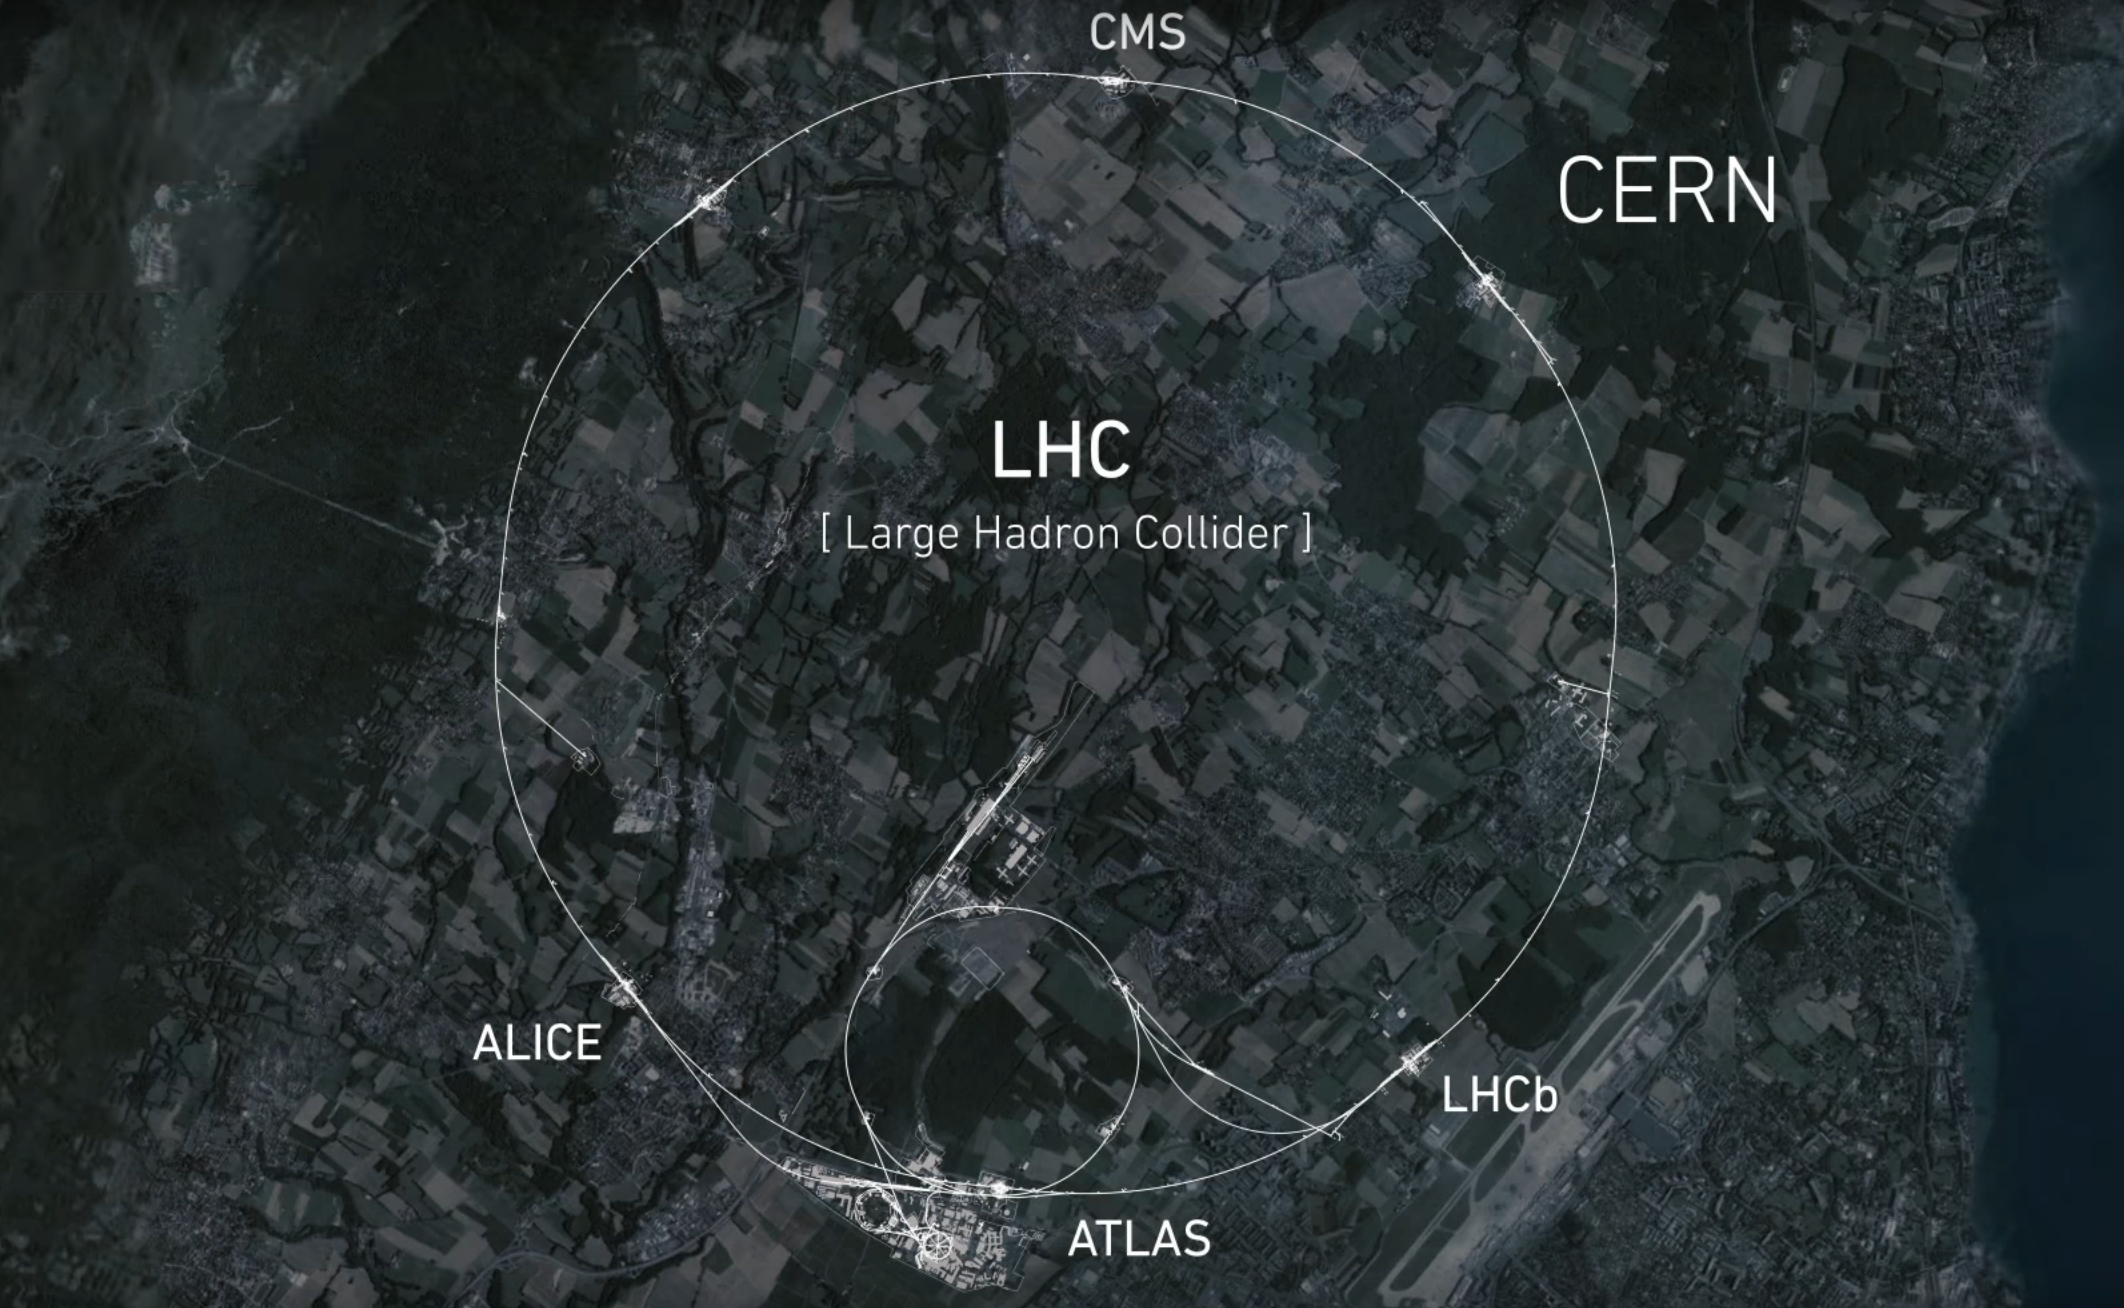
\includegraphics[height=6.65cm]{\PhDthesisdir/plots_and_images/CERN_and_LHC/LHC_map2.png}};
%\draw [ultra thick, ltcolorred] (5.65,3.6) circle (3) ; %LHC
%\draw [ultra thick, ltcolorred] (5.325,1.375) circle (.775) ; % SPS
%\draw [ultra thick, ltcolorred] (5.025,0.34) circle (.075) ; % PS
%\fill [ltcolorred] (4.925,0.375) circle (.025) ; % Booster
%\draw [thick, ltcolorred] (4.925,0.375) --+ (-85:.1) ; % LINAC2
\node[anchor=south west,inner sep=0] at (.75,5) {
\includegraphics[height=1cm]{\PhDthesisdir/plots_and_images/misc_for_slides/flag-france.jpg}};
\node[anchor=south west,inner sep=0] at (9.5,.5) {
\includegraphics[height=1cm]{\PhDthesisdir/plots_and_images/misc_for_slides/flag-suisse.png}};
\end{tikzpicture}
\end{center}
\end{frame}

\begin{frame}\addtocounter{framenumber}{-1}
\frametitle{LHC}
\begin{center}
\begin{tikzpicture}[scale=.95]
\node[anchor=south west,inner sep=0] at (0,0) {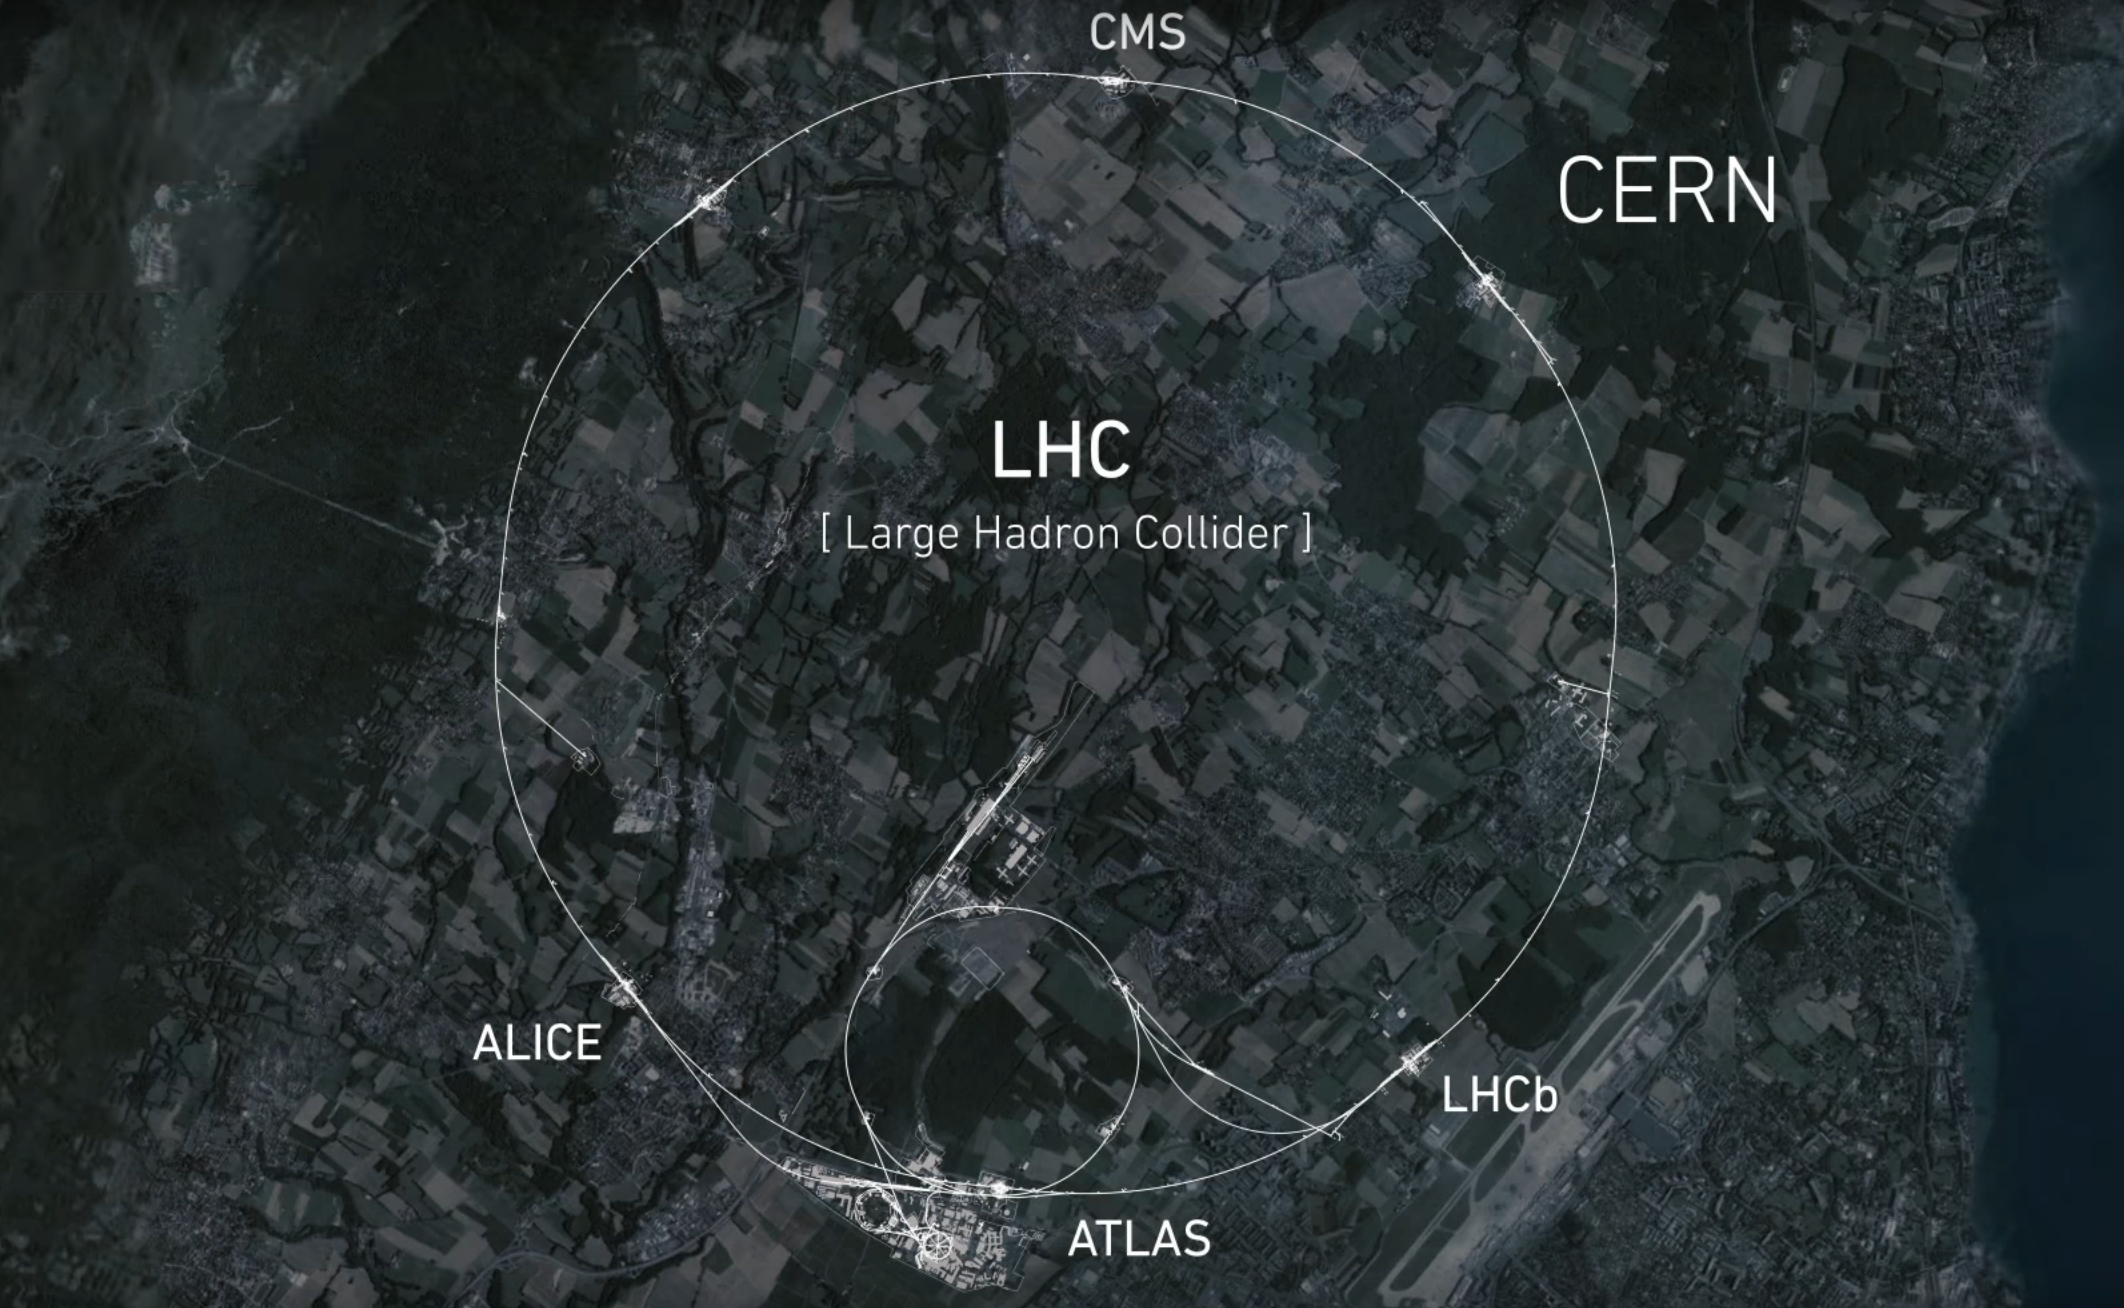
\includegraphics[height=6.65cm]{\PhDthesisdir/plots_and_images/CERN_and_LHC/LHC_map2.png}};
\draw [ultra thick, ltcolorred] (5.65,3.6) circle (3) ; %LHC
%\draw [ultra thick, ltcolorred] (5.325,1.375) circle (.775) ; % SPS
%\draw [ultra thick, ltcolorred] (5.025,0.34) circle (.075) ; % PS
%\fill [ltcolorred] (4.925,0.375) circle (.025) ; % Booster
%\draw [thick, ltcolorred] (4.925,0.375) --+ (-85:.1) ; % LINAC2
\end{tikzpicture}
\end{center}
\end{frame}

\begin{frame}\addtocounter{framenumber}{-1}
\frametitle{LINAC2 (\SI{50}{\MeV})}
\begin{center}
\begin{tikzpicture}[scale=.95]
\node[anchor=south west,inner sep=0] at (0,0) {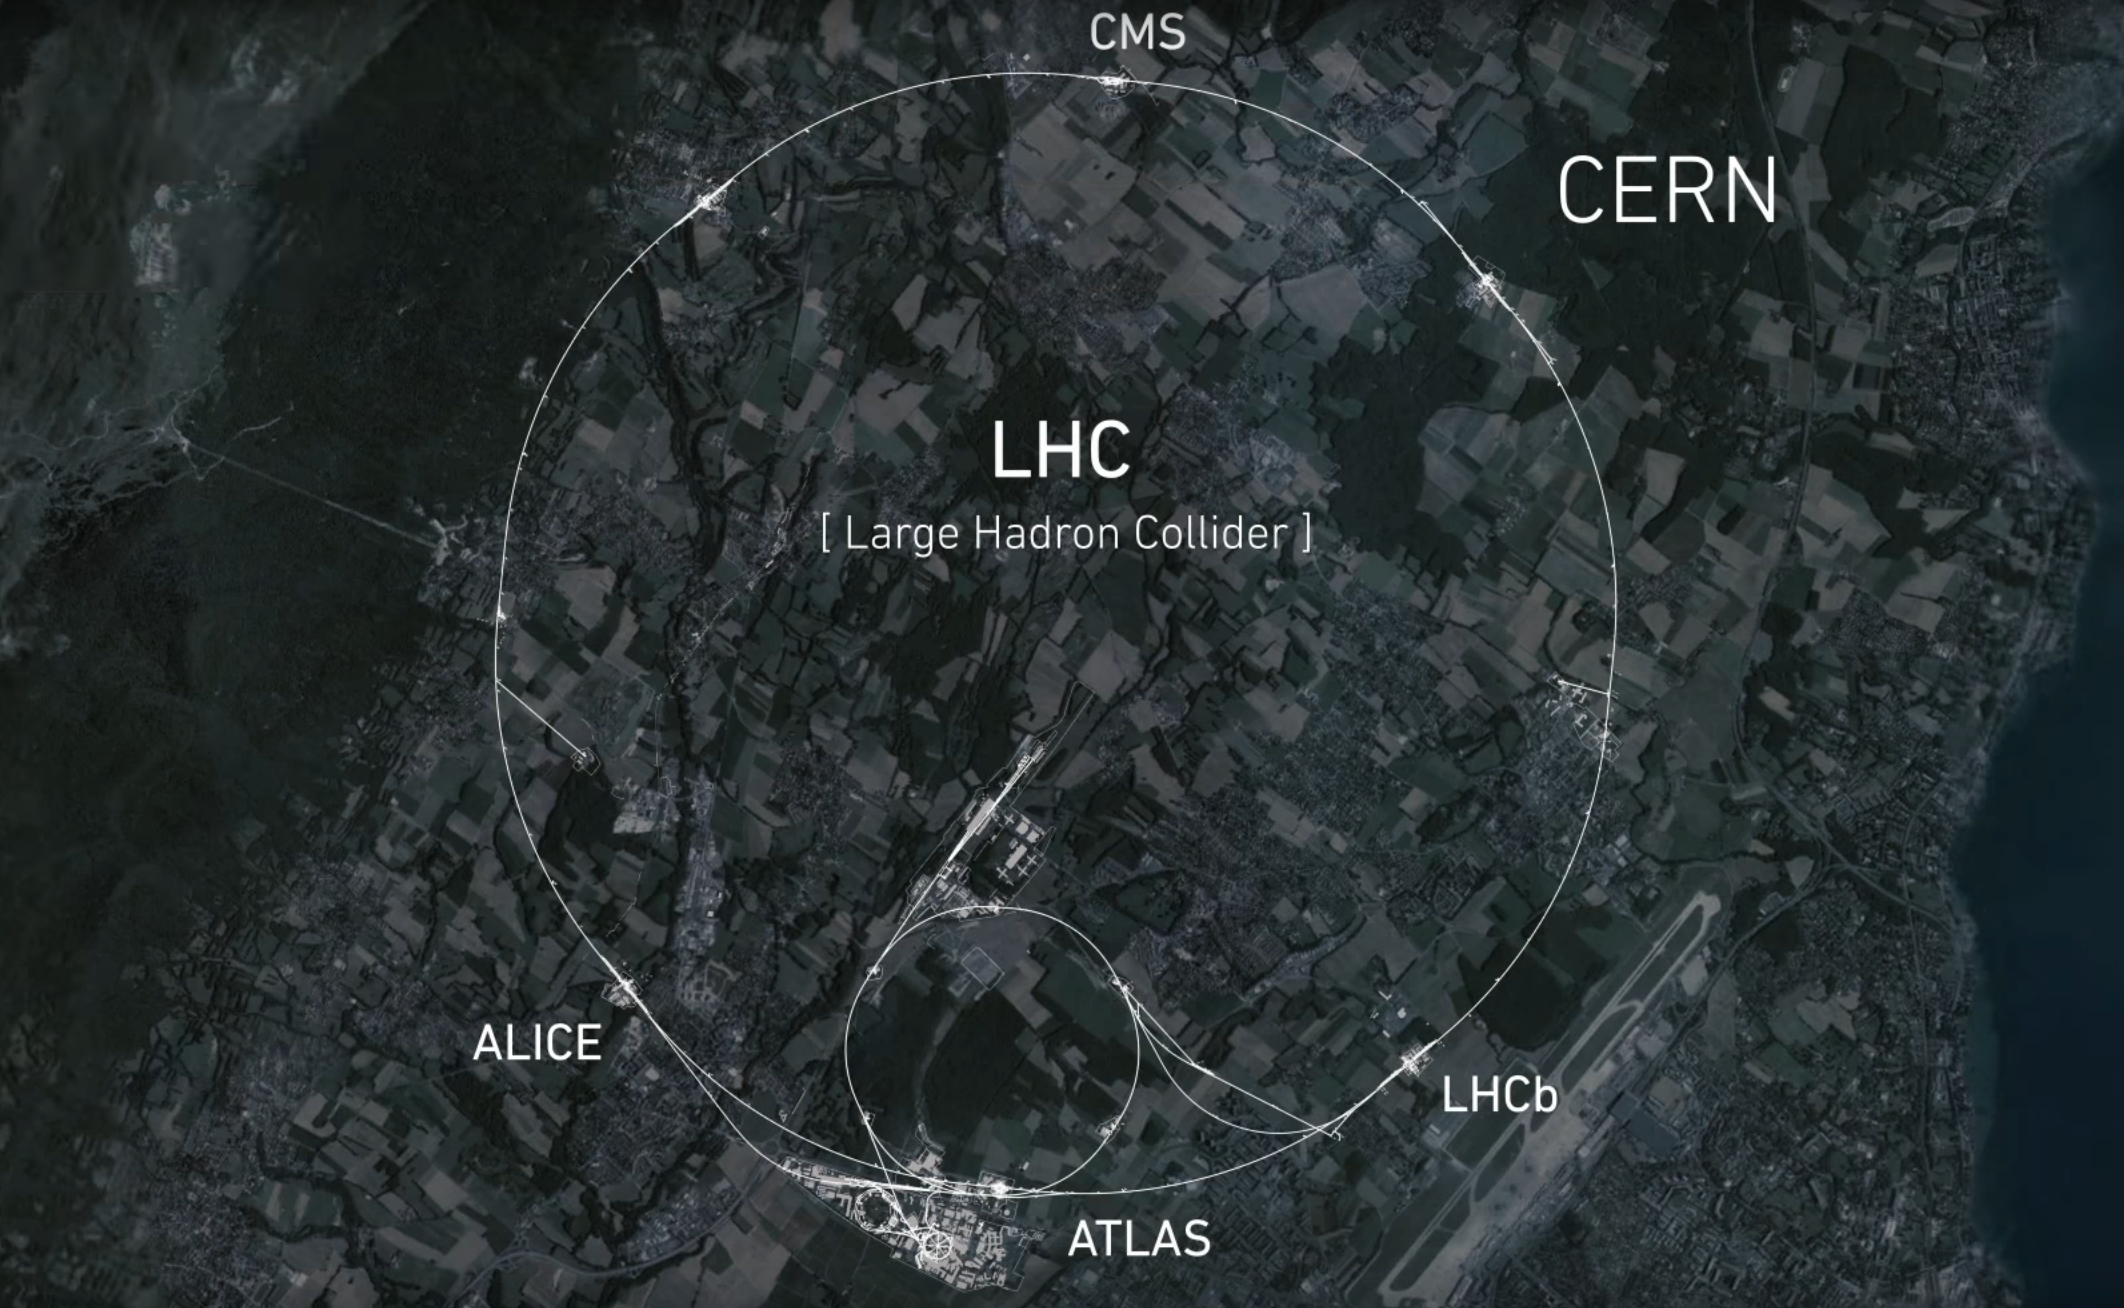
\includegraphics[height=6.65cm]{\PhDthesisdir/plots_and_images/CERN_and_LHC/LHC_map2.png}};
%\draw [ultra thick, ltcolorred] (5.65,3.6) circle (3) ; %LHC
%\draw [ultra thick, ltcolorred] (5.325,1.375) circle (.775) ; % SPS
%\draw [ultra thick, ltcolorred] (5.025,0.34) circle (.075) ; % PS
%\fill [ltcolorred] (4.925,0.375) circle (.025) ; % Booster
\draw [thick, ltcolorred] (4.925,0.375) --+ (-85:.1) ; % LINAC2
\draw [ultra thick, ltcolorred, latex-] (4.925,0.375) --+ (170:3) ;
\end{tikzpicture}
\end{center}
\end{frame}

\begin{frame}\addtocounter{framenumber}{-1}
\frametitle{Booster (1972, \SI{157}{\meter}, \SI{1.4}{\GeV})}
\begin{center}
\begin{tikzpicture}[scale=.95]
\node[anchor=south west,inner sep=0] at (0,0) {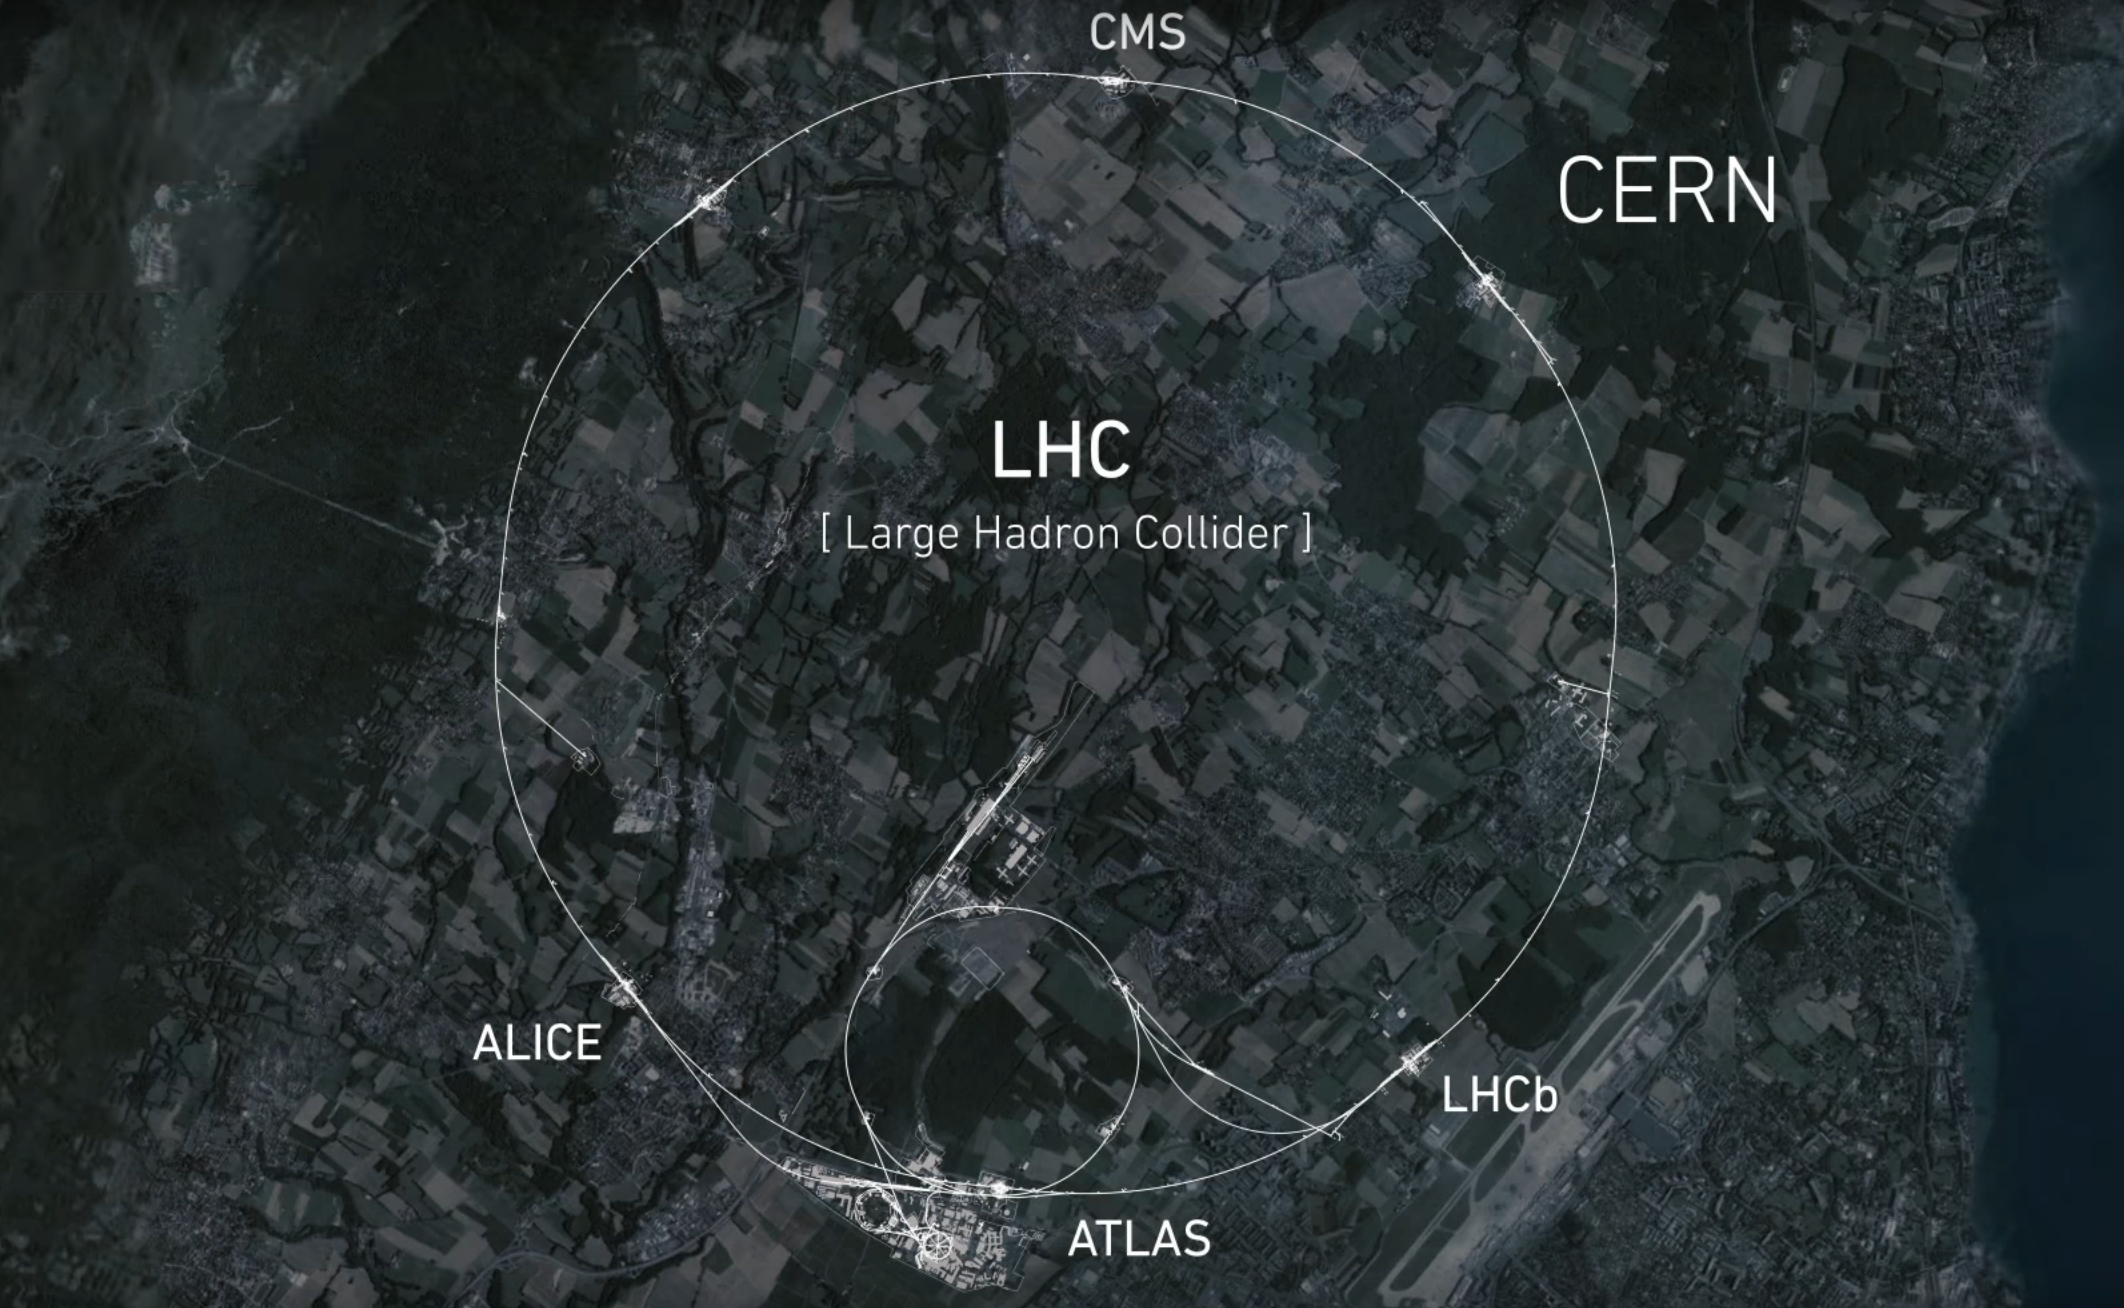
\includegraphics[height=6.65cm]{\PhDthesisdir/plots_and_images/CERN_and_LHC/LHC_map2.png}};
%\draw [ultra thick, ltcolorred] (5.65,3.6) circle (3) ; %LHC
%\draw [ultra thick, ltcolorred] (5.325,1.375) circle (.775) ; % SPS
%\draw [ultra thick, ltcolorred] (5.025,0.34) circle (.075) ; % PS
\fill [ltcolorred] (4.925,0.375) circle (.025) ; % Booster
%\draw [thick, ltcolorred] (4.925,0.375) --+ (-85:.1) ; % LINAC2
\draw [ultra thick, ltcolorred, latex-] (4.925,0.375) --+ (170:3) ;
\end{tikzpicture}
\end{center}
\end{frame}

\begin{frame}\addtocounter{framenumber}{-1}
\frametitle{PS (1959, \SI{628}{\meter}, \SI{25}{\GeV})}
\begin{center}
\begin{tikzpicture}[scale=.95]
\node[anchor=south west,inner sep=0] at (0,0) {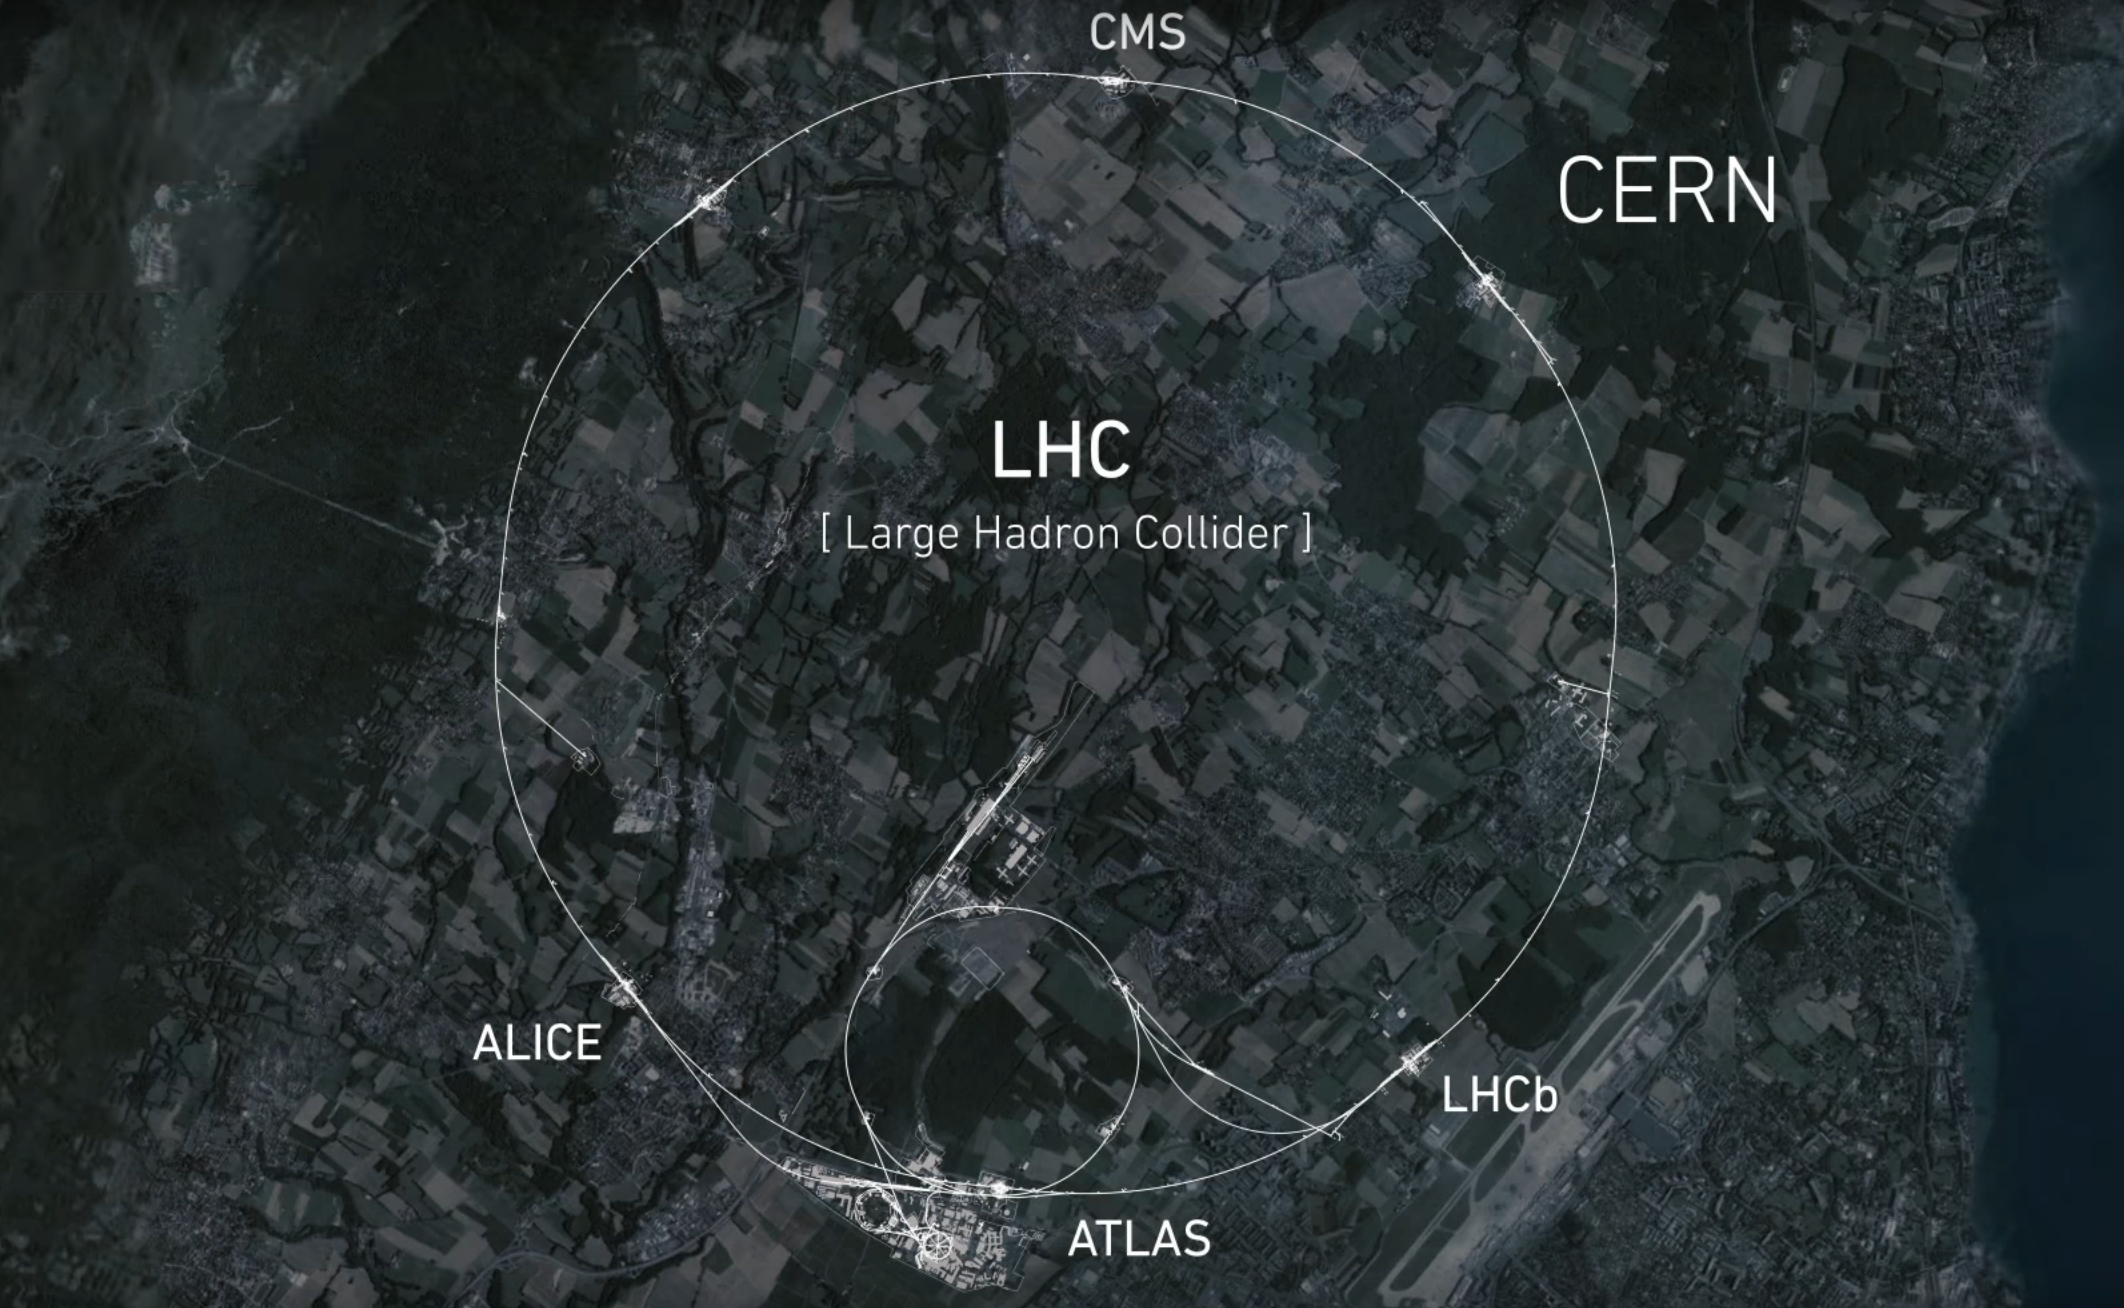
\includegraphics[height=6.65cm]{\PhDthesisdir/plots_and_images/CERN_and_LHC/LHC_map2.png}};
%\draw [ultra thick, ltcolorred] (5.65,3.6) circle (3) ; %LHC
%\draw [ultra thick, ltcolorred] (5.325,1.375) circle (.775) ; % SPS
\draw [ultra thick, ltcolorred] (5.025,0.34) circle (.075) ; % PS
%\fill [ltcolorred] (4.925,0.375) circle (.025) ; % Booster
%\draw [thick, ltcolorred] (4.925,0.375) --+ (-85:.1) ; % LINAC2
\draw [ultra thick, ltcolorred, latex-] (4.925,0.375) --+ (170:3) ;
\end{tikzpicture}
\end{center}
\end{frame}

\begin{frame}\addtocounter{framenumber}{-1}
\frametitle{SPS (1976, \SI{7}{\kilo\meter}, \SI{450}{\GeV})}
\begin{center}
\begin{tikzpicture}[scale=.95]
\node[anchor=south west,inner sep=0] at (0,0) {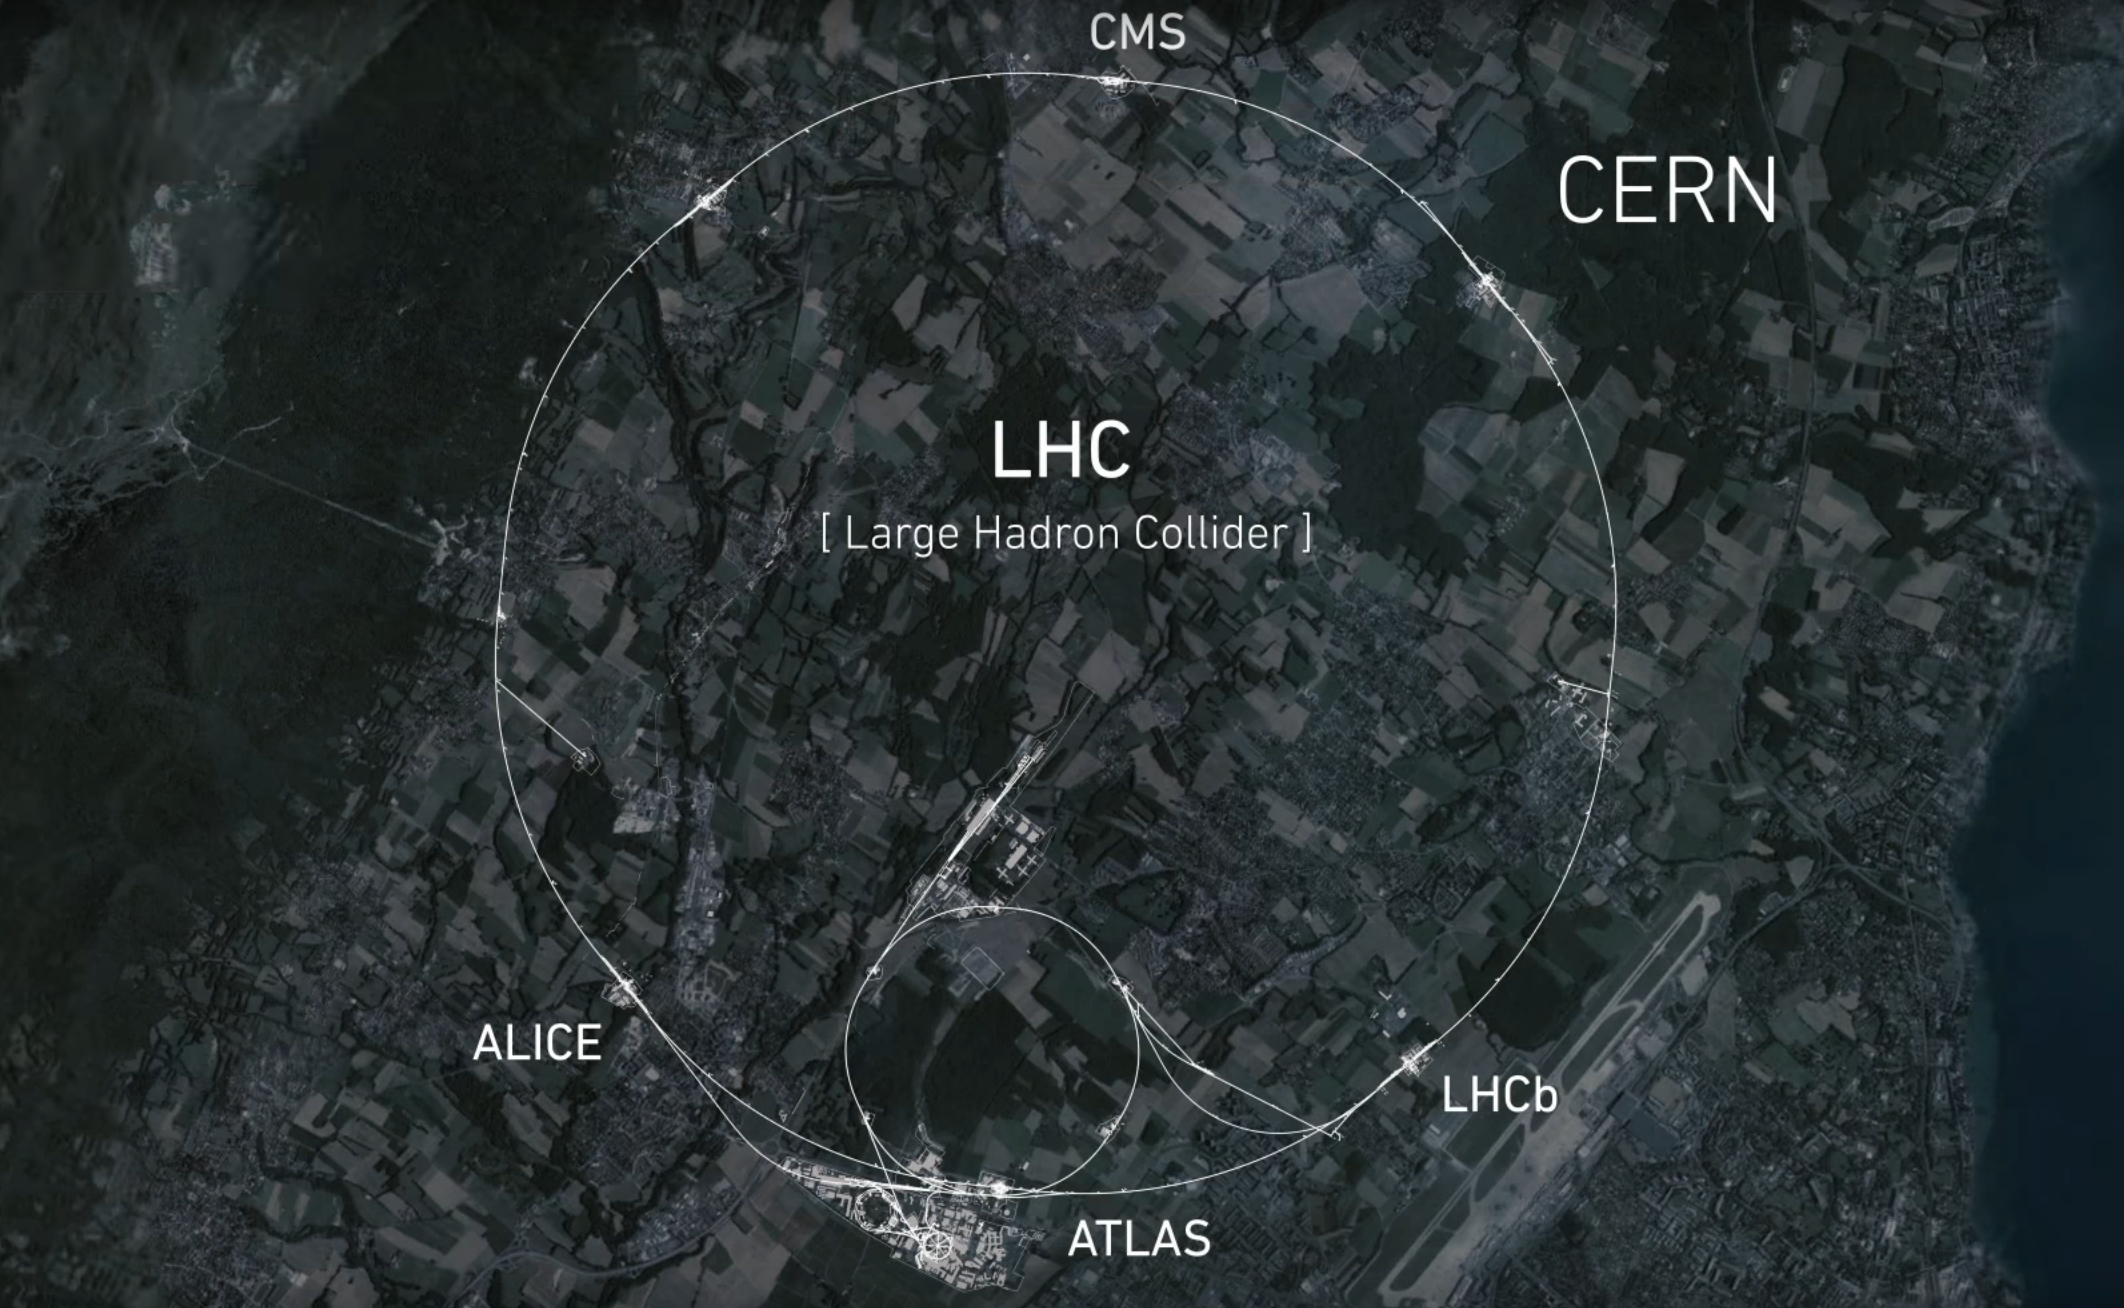
\includegraphics[height=6.65cm]{\PhDthesisdir/plots_and_images/CERN_and_LHC/LHC_map2.png}};
%\draw [ultra thick, ltcolorred] (5.65,3.6) circle (3) ; %LHC
\draw [ultra thick, ltcolorred] (5.325,1.375) circle (.775) ; % SPS
%\draw [ultra thick, ltcolorred] (5.025,0.34) circle (.075) ; % PS
%\fill [ltcolorred] (4.925,0.375) circle (.025) ; % Booster
%\draw [thick, ltcolorred] (4.925,0.375) --+ (-85:.1) ; % LINAC2
\end{tikzpicture}
\end{center}
\end{frame}

\begin{frame}\addtocounter{framenumber}{-1}
\frametitle{LHC (2008, \SI{27}{\kilo\meter}, $2\times\SI{7}{\TeV}$)}
\begin{center}
\begin{tikzpicture}[scale=.95]
\node[anchor=south west,inner sep=0] at (0,0) {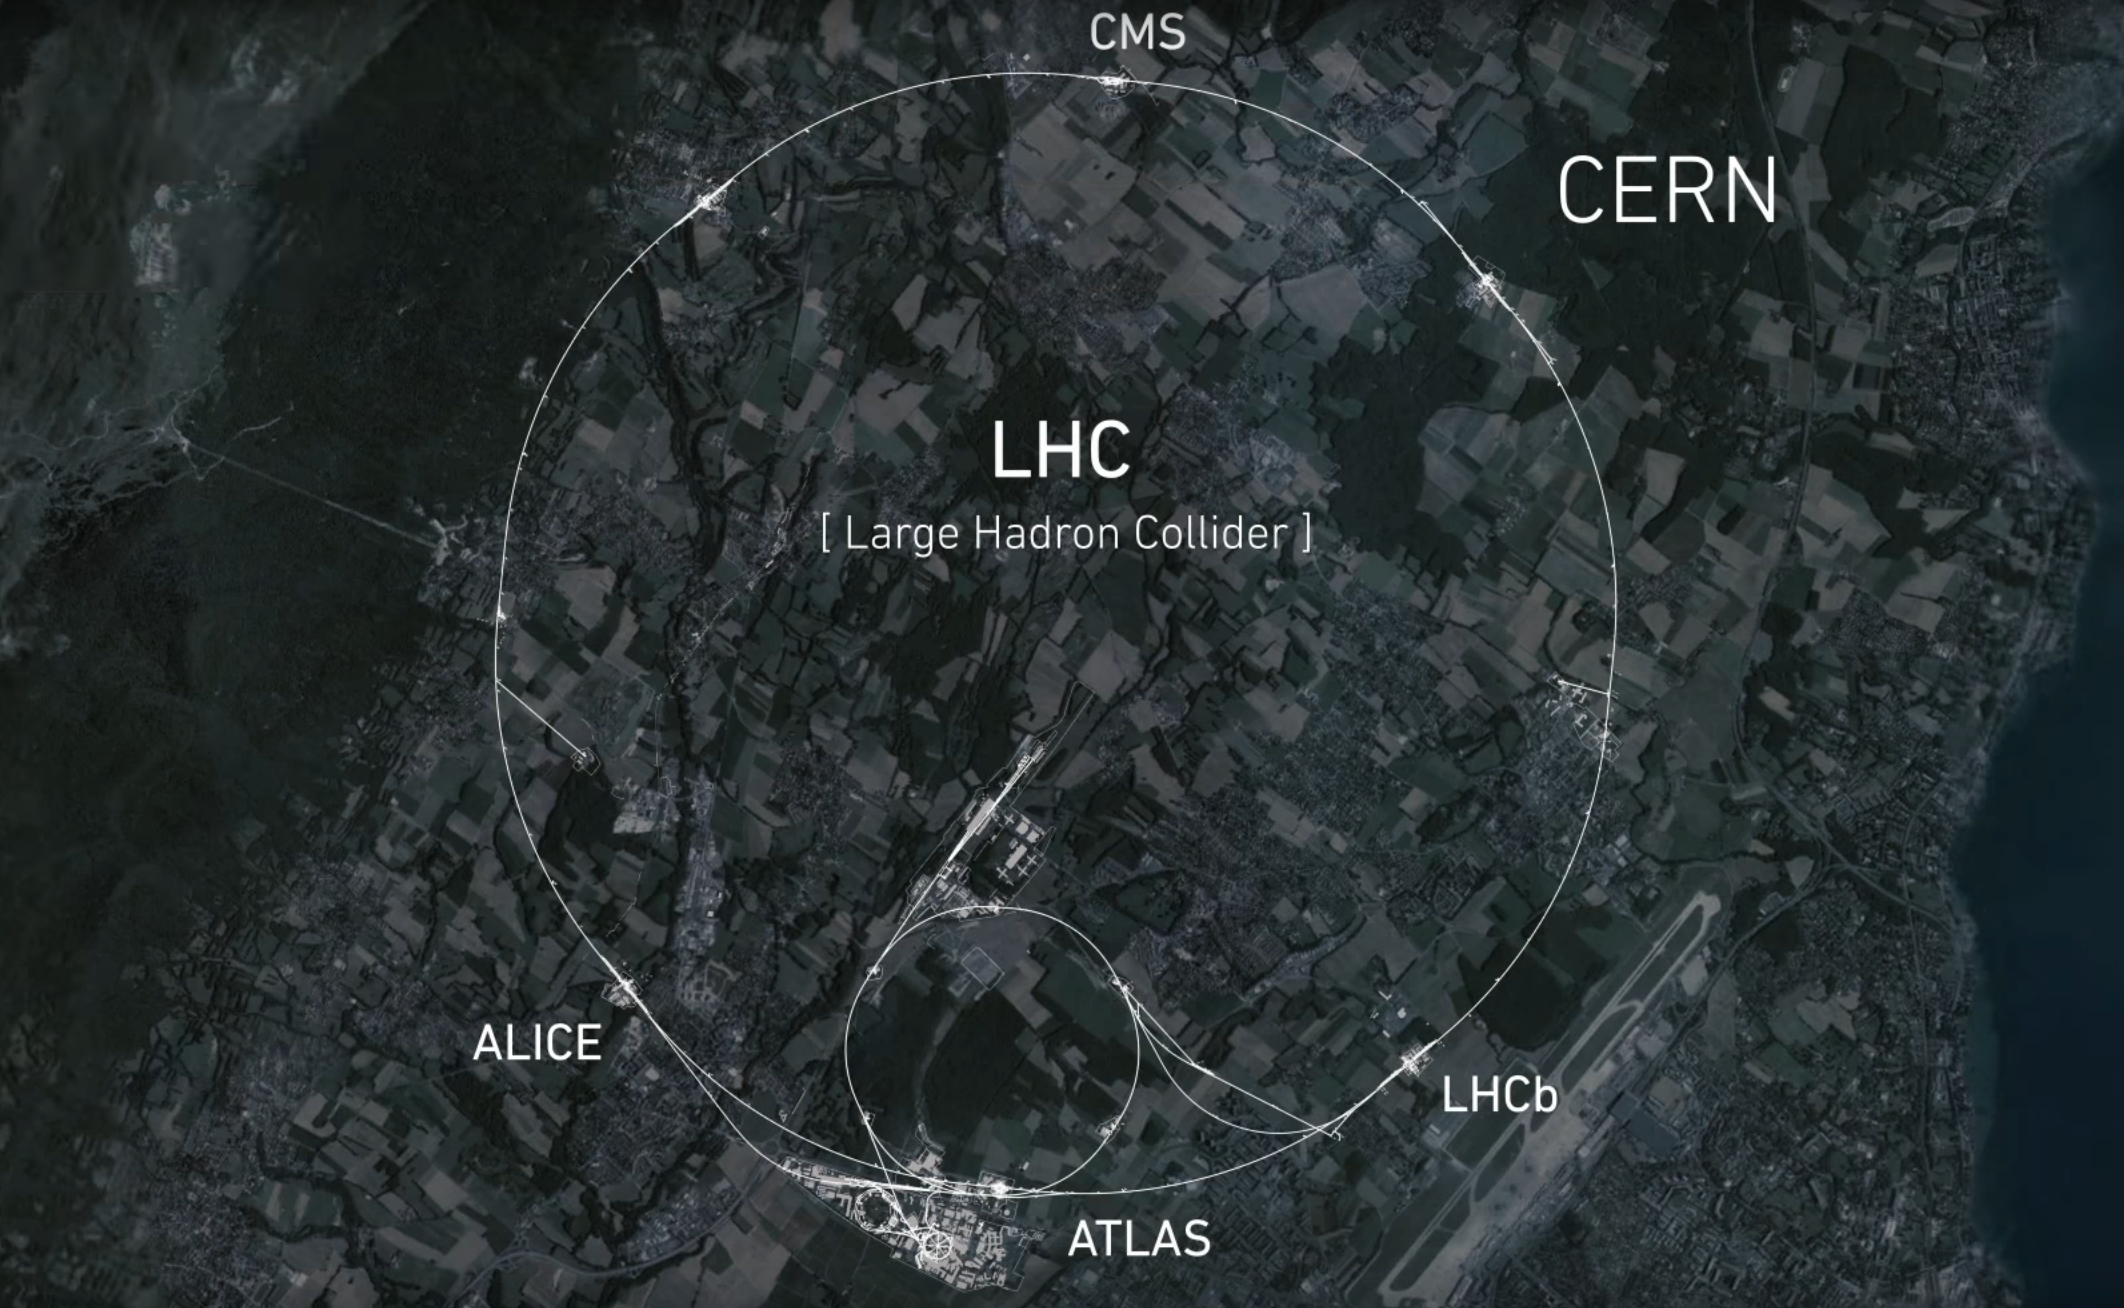
\includegraphics[height=6.65cm]{\PhDthesisdir/plots_and_images/CERN_and_LHC/LHC_map2.png}};
\draw [ultra thick, ltcolorred] (5.65,3.6) circle (3) ; %LHC
%\draw [ultra thick, ltcolorred] (5.325,1.375) circle (.775) ; % SPS
%\draw [ultra thick, ltcolorred] (5.025,0.34) circle (.075) ; % PS
%\fill [ltcolorred] (4.925,0.375) circle (.025) ; % Booster
%\draw [thick, ltcolorred] (4.925,0.375) --+ (-85:.1) ; % LINAC2
\end{tikzpicture}
\end{center}
\end{frame}
\begin{frame}
\frametitle{CERN LHC}

\begin{minipage}[c]{.45\textwidth}
\begin{center}
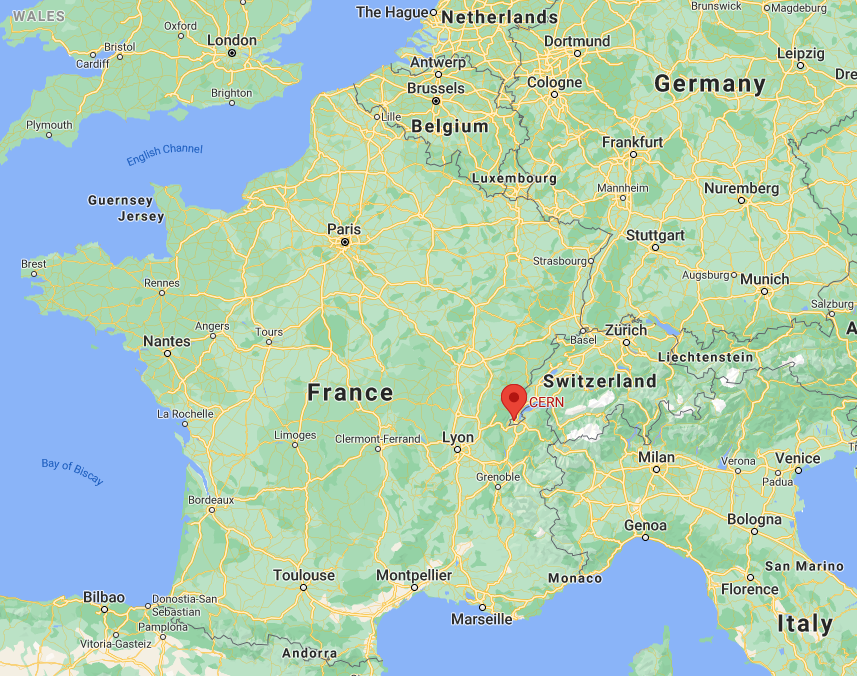
\includegraphics[width=.99\textwidth]{\PhDthesisdir/plots_and_images/CERN_and_LHC/maps-en.png}
\end{center}
\end{minipage}
\hfill
\begin{minipage}[c]{.5\textwidth}
\begin{center}
\begin{tikzpicture}
\node[anchor=south west,inner sep=0] at (0,0) {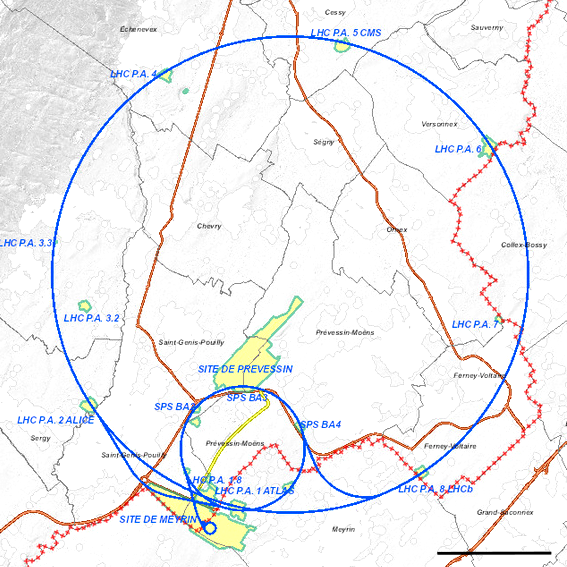
\includegraphics[scale=.35]{\PhDthesisdir/slides/LHC-CMS/LHC/CERN_LHC_map-scale_2km.png}};
\draw (6.125,.4) node {\SI{2}{\kilo\meter}};
\draw (2.95,.75) coordinate (LHCp1);
\draw (1.125,2) coordinate (LHCp2);
\draw (.65,4) coordinate (LHCp3);
\draw (1,3.2) coordinate (LHCp32);
\draw (2,6.1) coordinate (LHCp4);
\draw (4.25,6.45) coordinate (LHCp5);
\draw (6.05,5.15) coordinate (LHCp6);
\draw (6.15,3.125) coordinate (LHCp7);
\draw (5.15,1.15) coordinate (LHCp8);
\draw (LHCp1) coordinate (ATLAS);
\draw (LHCp2) coordinate (ALICE);
\draw (LHCp5) coordinate (CMS);
\draw (LHCp8) coordinate (LHCb);

%\foreach \coord in {1,2,3,4,5,6,7,8,32}{
%\fill[ltcolorred] (LHCp\coord) circle (3pt);
%}

%\draw [ultra thick, ltcolorred] (3.575,3.625) circle (2.95) ;
%\draw [ultra thick, ltcolorred] (3,1.475) circle (.75) ;
%\draw [ultra thick, ltcolorred] (2.6,.5) circle (.075) ;
%\fill [ltcolorred] (2.55,.55) circle (.05) ;
%\draw [ultra thick, ltcolorred] (2.5,.5) --+ (-60:.15) ;
\fill[ltcolorred] (CMS) circle (3pt);
\draw [ltcolorred4] (CMS) node [below] {\textbf{CMS}};
\fill[ltcolorred] (ATLAS) circle (3pt);
\draw [ltcolorred4] (ATLAS) node [above] {\textbf{ATLAS}};
\fill[ltcolorred] (ALICE) circle (3pt);
\draw [ltcolorred4] (ALICE) node [above right] {\textbf{ALICE}};
\fill[ltcolorred] (LHCb) circle (3pt);
\draw [ltcolorred4] (LHCb) node [below right] {\textbf{LHCb}};
\end{tikzpicture}
\end{center}
\end{minipage}
\end{frame}


\subsection*{The CMS detector}

\begin{frame}
\begin{center}
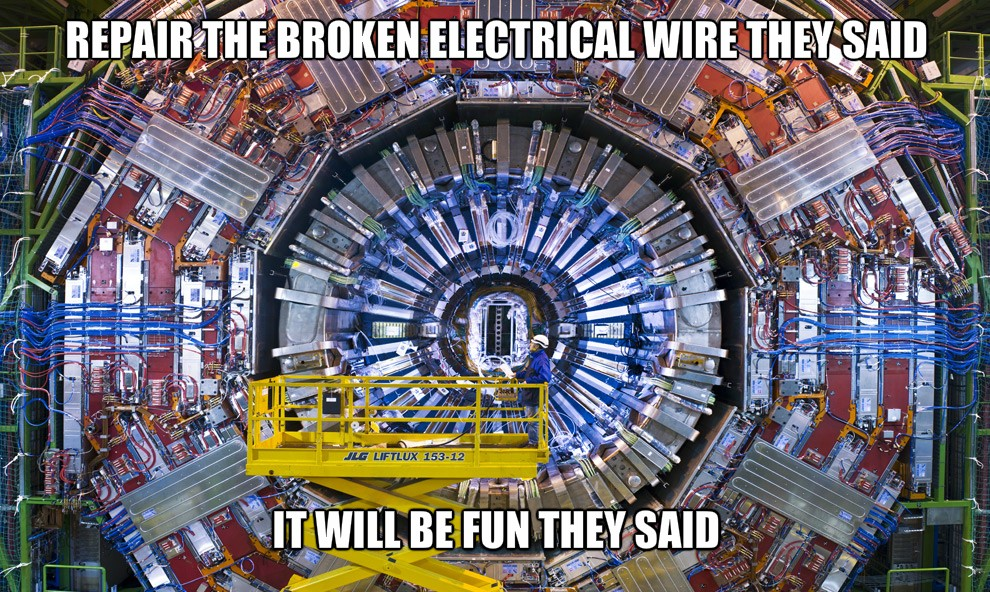
\includegraphics[width=\textwidth, height=\textheight, keepaspectratio]{\PhDthesisdir/plots_and_images/CMS_slices/how-do-you-do-when-lhc-is-broken_o_2241667.jpg}
\end{center}
\end{frame}


%\begin{frame}
\frametitle{The CMS detector}
\end{frame}
\begin{frame}\addtocounter{framenumber}{-1}
\frametitle{The CMS detector -- Silicon tracker (pixels)}
\begin{center}
detects charged particles going through

\vfill

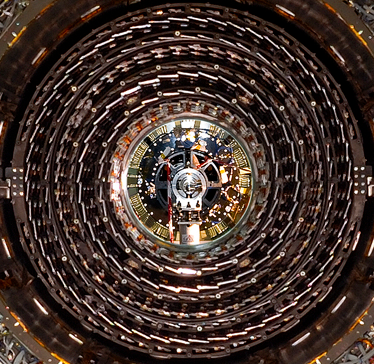
\includegraphics[width=\textwidth,height=0.75\textheight,keepaspectratio]{\PhDthesisdir/slides/LHC-CMS/CMS/CMS_zoomout_pictures/CMS_slice_photo_1-trk1.png}

\vfill

$\longleftarrow \SI{1}{\meter} \longrightarrow$
\end{center}
\end{frame}
\begin{frame}\addtocounter{framenumber}{-1}
\frametitle{The CMS detector -- Silicon tracker (strips)}
\begin{center}
detects charged particles going through

\vfill

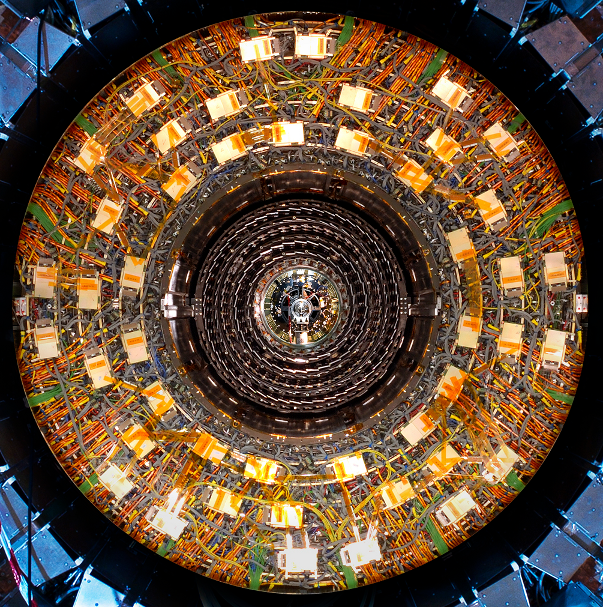
\includegraphics[width=\textwidth,height=0.75\textheight,keepaspectratio]{\PhDthesisdir/slides/LHC-CMS/CMS/CMS_zoomout_pictures/CMS_slice_photo_2-trk2.png}

\vfill

$\longleftarrow \SI{2}{\meter} \longrightarrow$
\end{center}
\end{frame}
\begin{frame}\addtocounter{framenumber}{-1}
\frametitle{The CMS detector -- Electromagnetic calorimeter (ECAL)}
\begin{center}
stops photons and electrons, measure their energies

\vfill

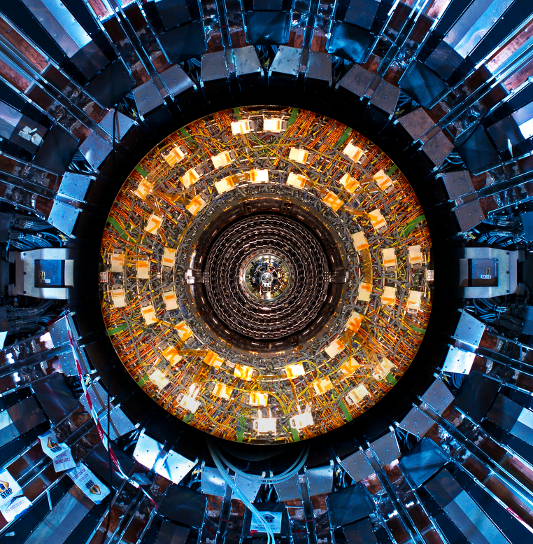
\includegraphics[width=\textwidth,height=0.75\textheight,keepaspectratio]{\PhDthesisdir/slides/LHC-CMS/CMS/CMS_zoomout_pictures/CMS_slice_photo_3-ECAL.png}

\vfill

$\longleftarrow \SI{3}{\meter} \longrightarrow$
\end{center}
\end{frame}
\begin{frame}\addtocounter{framenumber}{-1}
\frametitle{The CMS detector -- Hadron calorimeter (HCAL)}
\begin{center}
stops hadrons (protons, neutrons, ...), measure their energies

\vfill

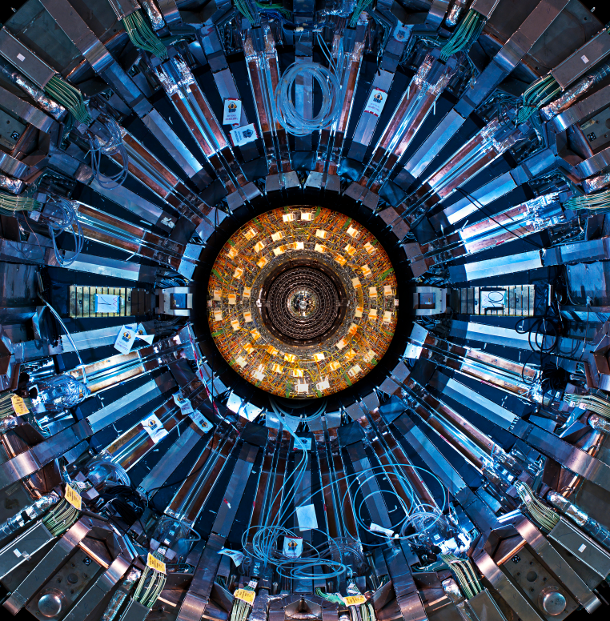
\includegraphics[width=\textwidth,height=0.75\textheight,keepaspectratio]{\PhDthesisdir/slides/LHC-CMS/CMS/CMS_zoomout_pictures/CMS_slice_photo_4-HCAL.png}

\vfill

$\longleftarrow \SI{5}{\meter} \longrightarrow$
\end{center}
\end{frame}
\begin{frame}\addtocounter{framenumber}{-1}
\frametitle{The CMS detector -- Superconducting solenoid}
\begin{center}
creates a \SI{4}{\tesla} magnetic field which bends charged particles trajectories

\vfill

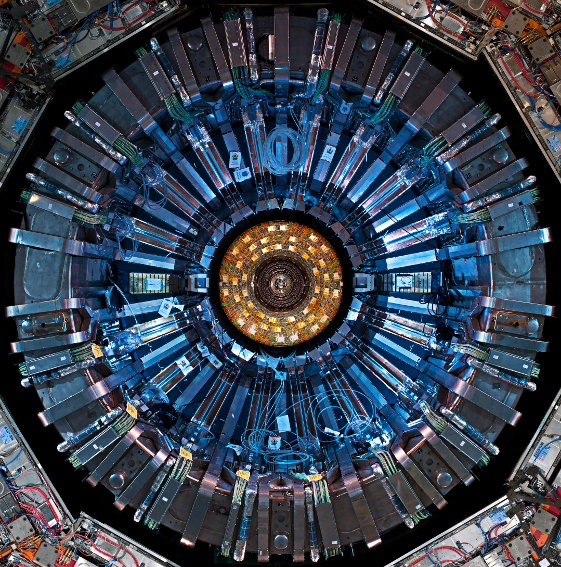
\includegraphics[width=\textwidth,height=0.75\textheight,keepaspectratio]{\PhDthesisdir/slides/LHC-CMS/CMS/CMS_zoomout_pictures/CMS_slice_photo_5-solenoid.png}

\vfill

$\longleftarrow \SI{7}{\meter} \longrightarrow$
\end{center}
\end{frame}
\begin{frame}\addtocounter{framenumber}{-1}
\frametitle{The CMS detector -- Muon system}
\begin{center}
detects muons going through

\vfill

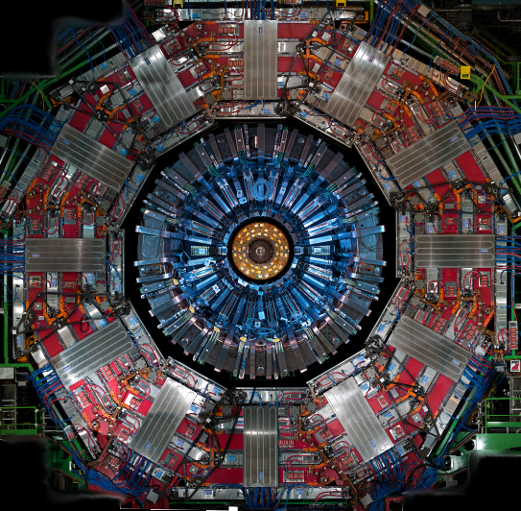
\includegraphics[width=\textwidth,height=0.75\textheight,keepaspectratio]{\PhDthesisdir/slides/LHC-CMS/CMS/CMS_zoomout_pictures/CMS_slice_photo_6-muons.png}

\vfill

$\longleftarrow \SI{15}{\meter} \longrightarrow$
\end{center}
\end{frame}
%\begin{frame}\addtocounter{framenumber}{-1}
\frametitle{The CMS detector}
\begin{center}
\vphantom{detects muons going through}

\vfill

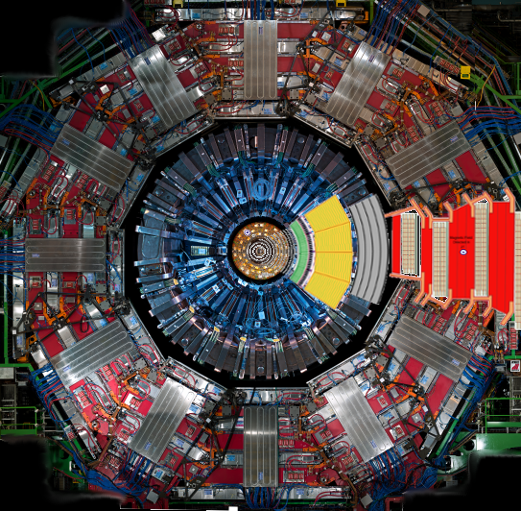
\includegraphics[width=\textwidth,height=0.75\textheight,keepaspectratio]{\PhDthesisdir/plots_and_images/CMS_slices/own/slice_on_photo.tex}

\vfill

$\longleftarrow \SI{15}{\meter} \longrightarrow$
\end{center}
\end{frame}
\begin{frame}
\begin{minipage}[t]{.6\textwidth}
\begin{figure}
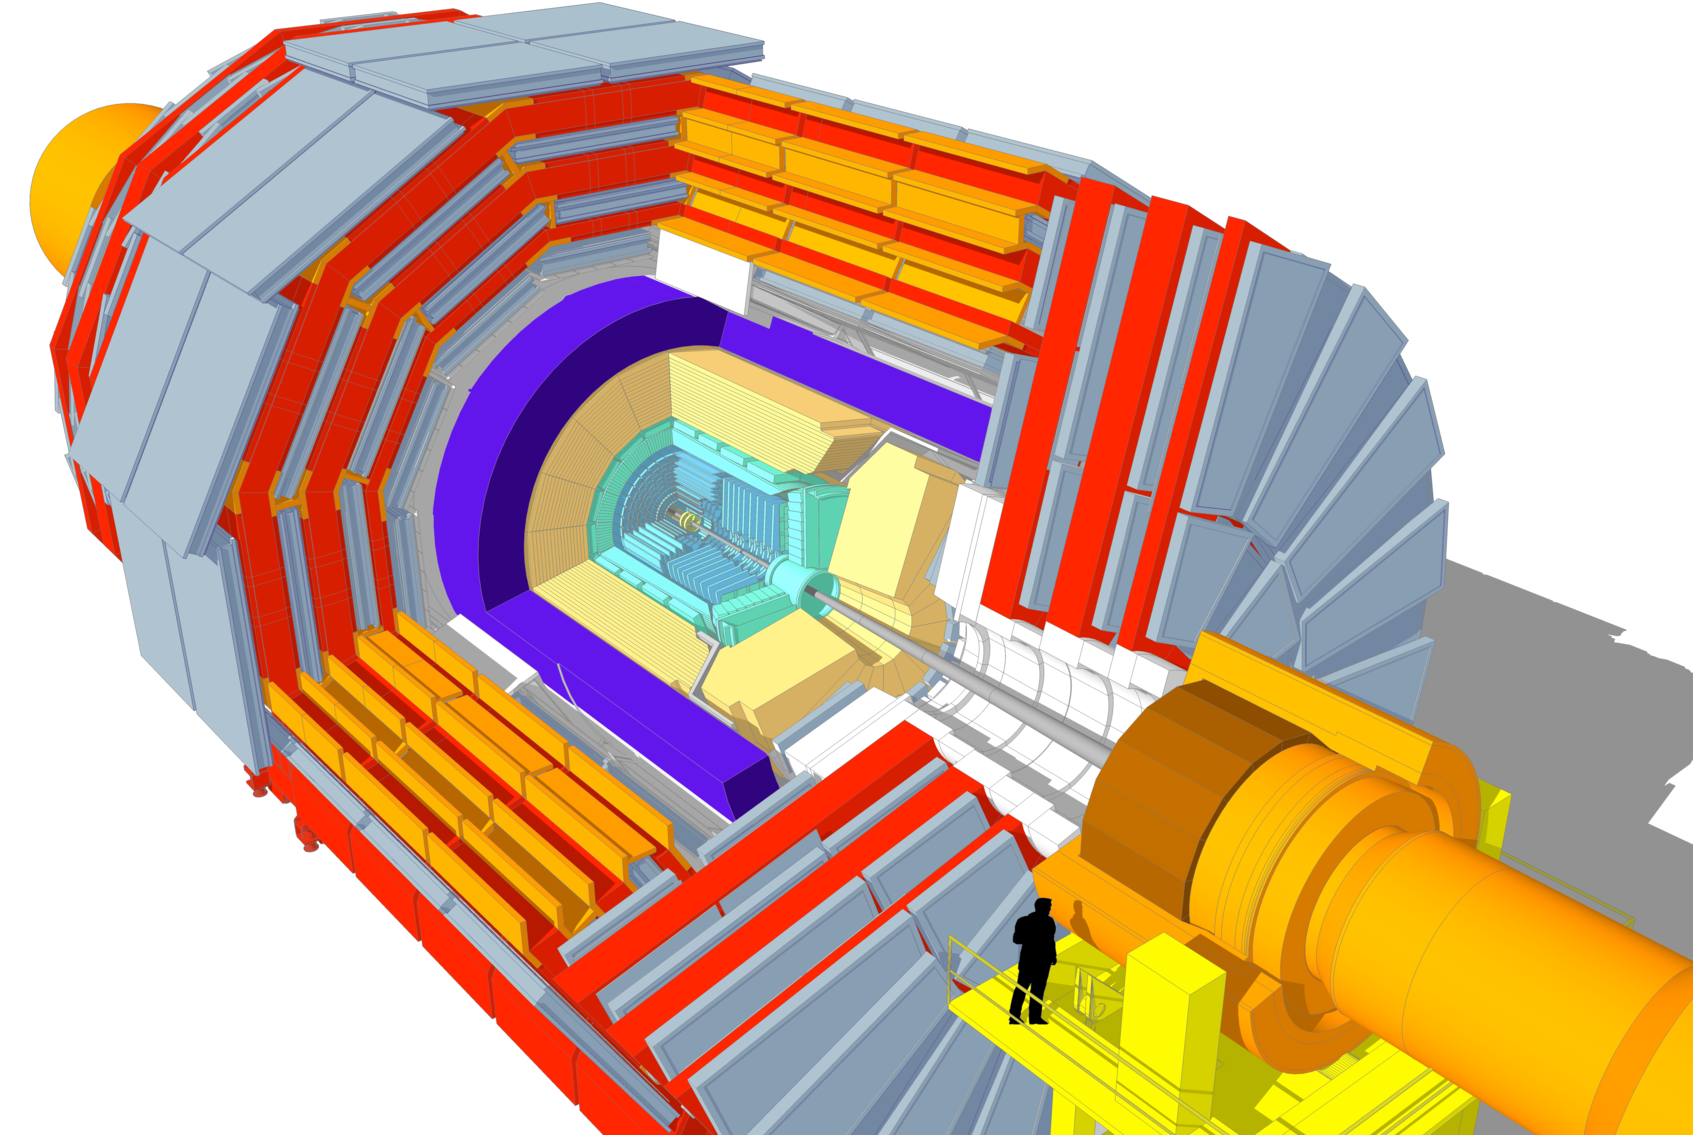
\includegraphics[width=\textwidth,height=\graphh,keepaspectratio]{\PhDthesisdir/plots_and_images/CMS_slices/from_CMS_document_11982-v2/small_cms_full.png}
\end{figure}
\end{minipage}
\hfill\begin{minipage}[t]{.35\textwidth}
\begin{block}{CMS detector}
\begin{itemize}
\item Mass: $\sim\SI{14000}{t}$, $\num{12500}$ only for red part
\item Diameter: \SI{15}{\meter}
\item Length: \SI{28.7}{\meter}
\end{itemize}
\end{block}

\begin{block}{}
$\Rightarrow$ How to \emph{see} the particles?
\end{block}
\end{minipage}
\end{frame}

\begin{frame}
\addtocounter{framenumber}{-1}
%\transdissolve
\begin{minipage}[t]{.6\textwidth}
\begin{figure}
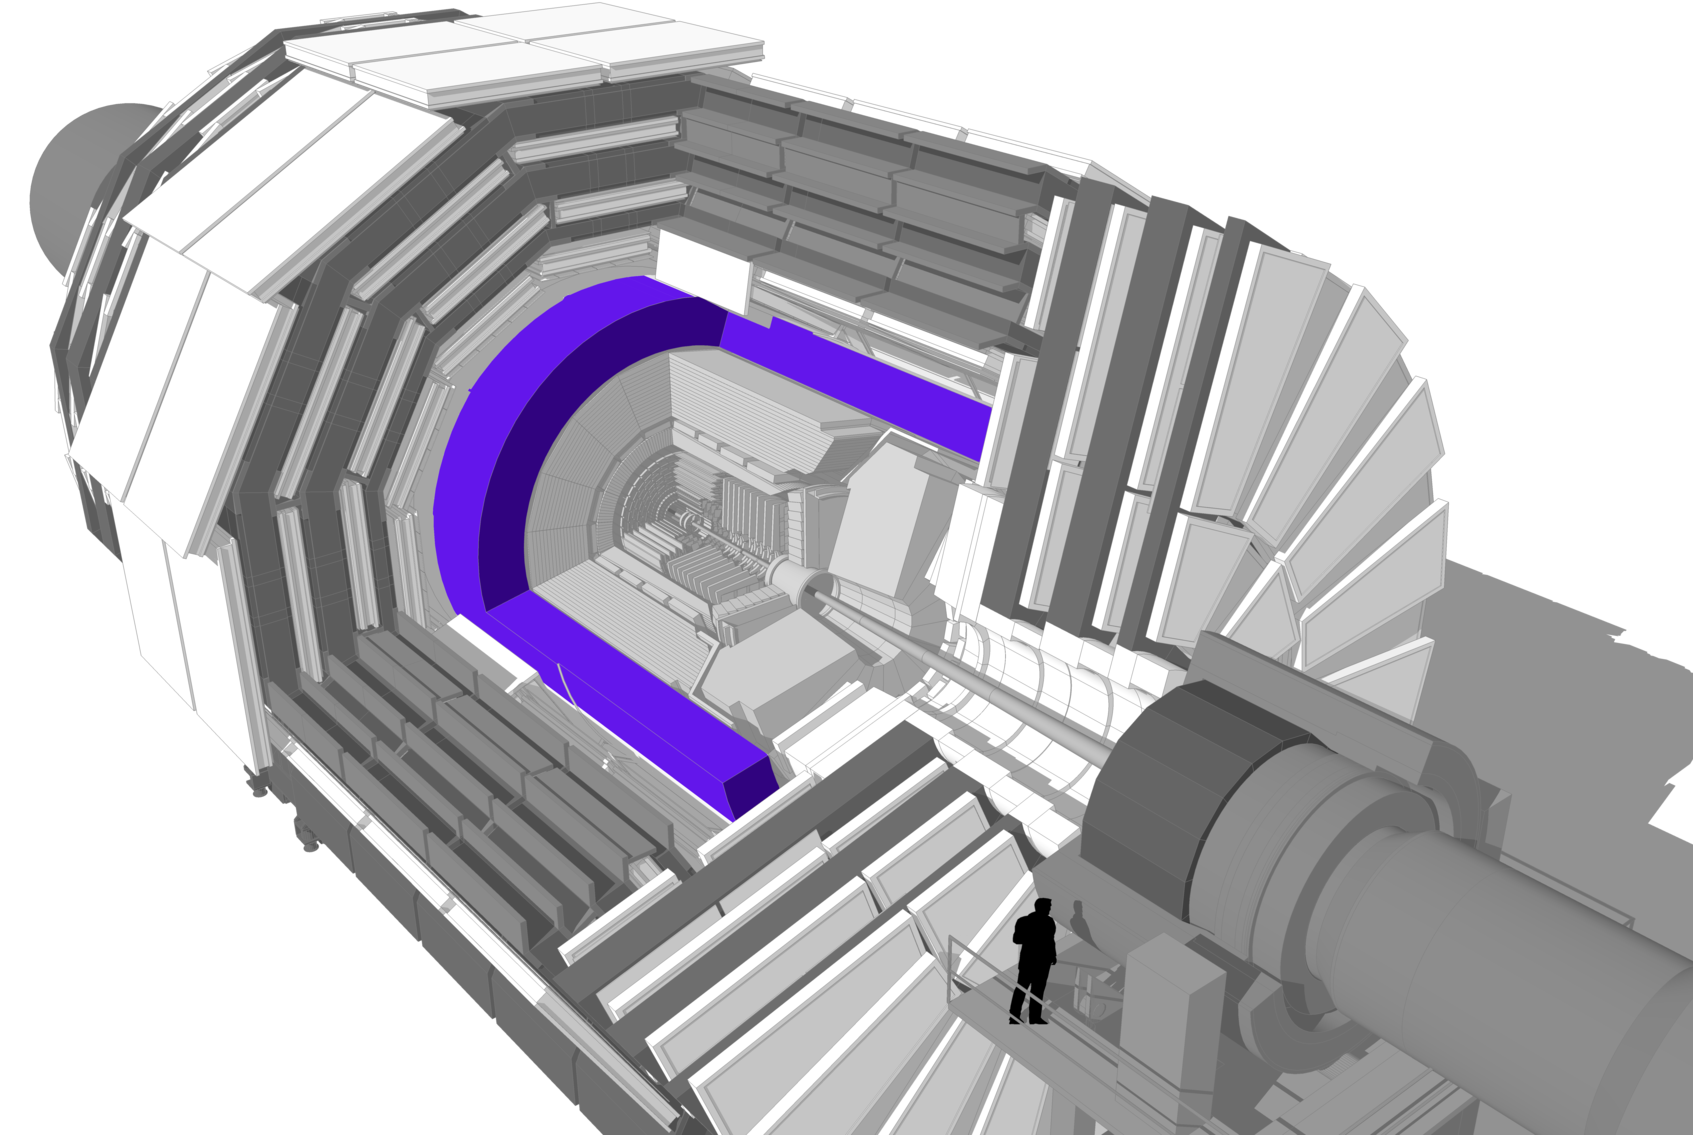
\includegraphics[width=\textwidth,height=\graphh,keepaspectratio]{\PhDthesisdir/plots_and_images/CMS_slices/from_CMS_document_11982-v2/small_cms_solenoid.png}
\end{figure}
\end{minipage}
\hfill\begin{minipage}[t]{.35\textwidth}
\begin{block}{Solenoid}
\begin{itemize}
\item Niobium titanium coil
\item Superconducting
\item $\sim\SI{18000}{\ampere}$
\item \SI{4}{\tesla} in the inner volume
\end{itemize}
\end{block}

\begin{block}{}
$\Rightarrow$ Bends charged particles trajectories in the transverse plane
\end{block}
\end{minipage}
\end{frame}

\begin{frame}
\addtocounter{framenumber}{-1}
%\transdissolve
\begin{minipage}[t]{.6\textwidth}
\begin{figure}
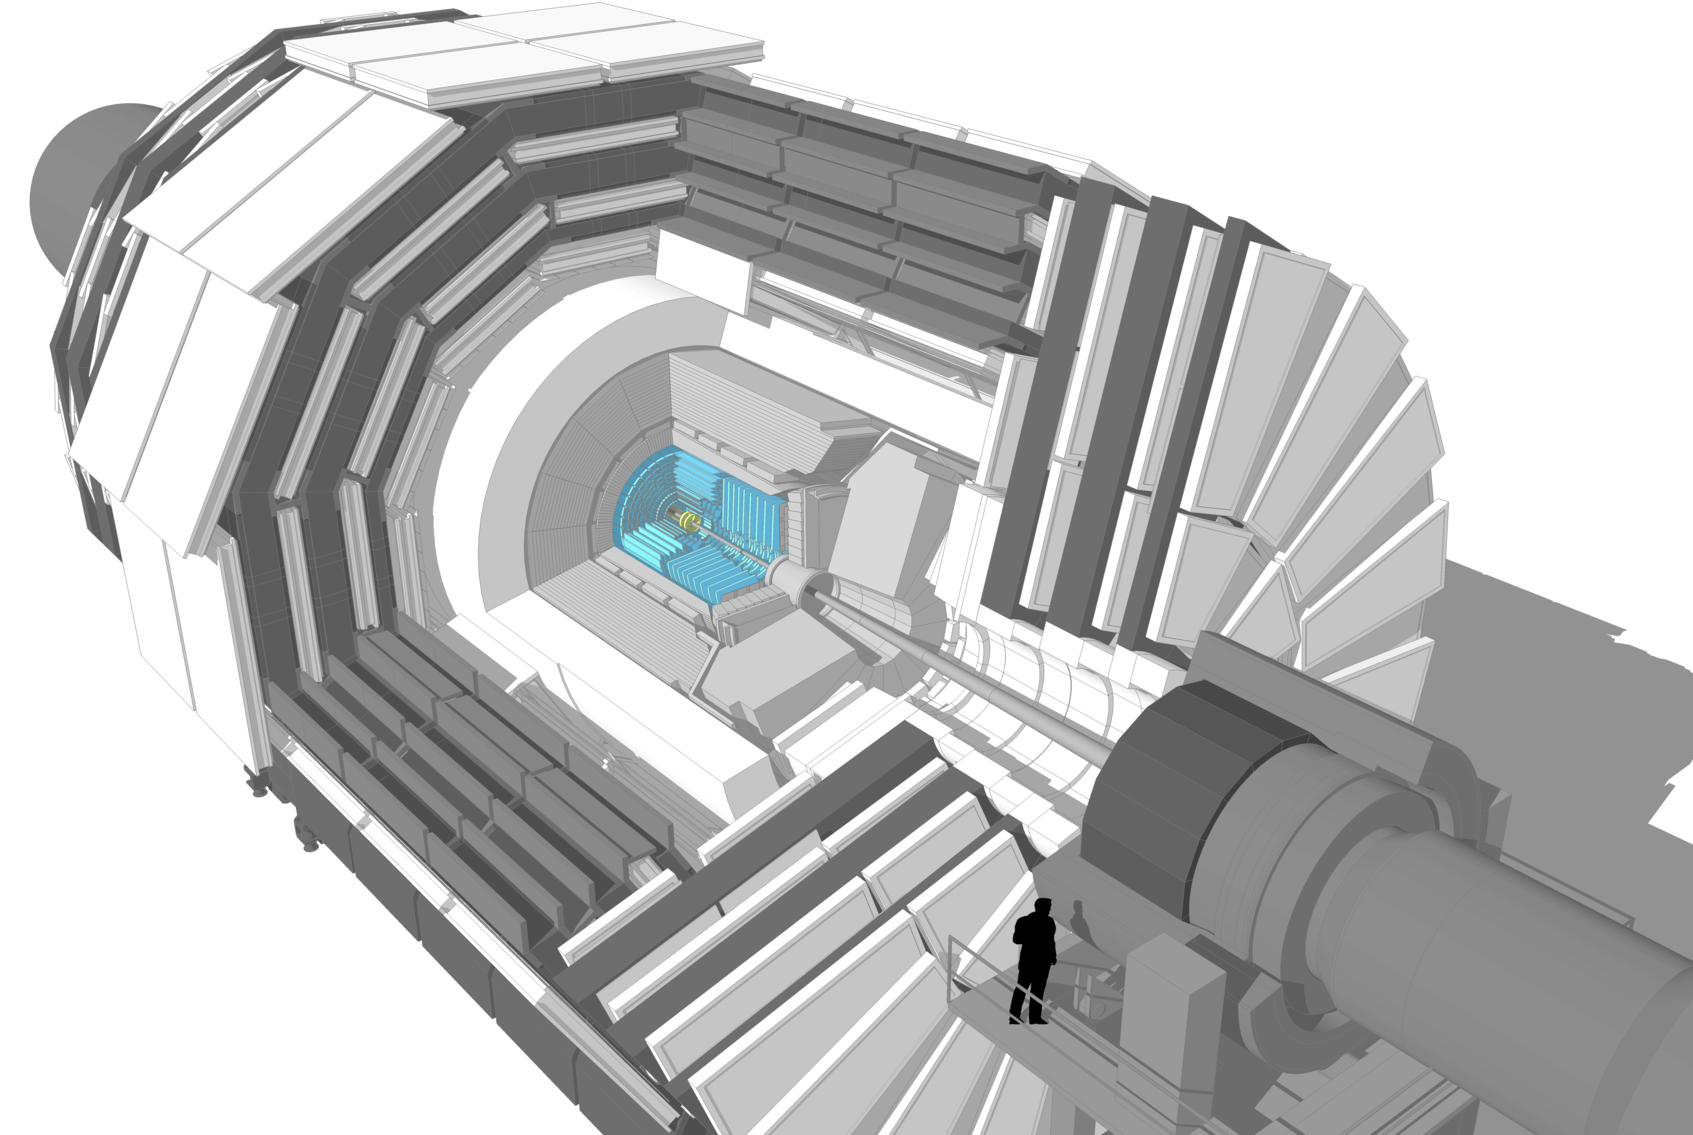
\includegraphics[width=\textwidth,height=\graphh,keepaspectratio]{\PhDthesisdir/plots_and_images/CMS_slices/from_CMS_document_11982-v2/small_cms_tracker.png}
\end{figure}
\end{minipage}
\hfill\begin{minipage}[t]{.35\textwidth}
\begin{block}{Tracker}
\begin{itemize}
\item Inner: pixels ($\num{100}\times\SI{150}{\micro\meter^2}$, $\sim\SI{1.9}{\meter^2}$, $\sim\SI{124}{M}$ channels
\item Outer: microstrips ($\num{80}-\SI{180}{\micro\meter}$) $\sim\SI{200}{\meter^2}$ $\sim\SI{9.6}{M}$ channels
\end{itemize}
\end{block}

\begin{block}{}
$\Rightarrow$ Charged particles leave hits when going through
\end{block}
\end{minipage}
\end{frame}

\begin{frame}
\addtocounter{framenumber}{-1}
%\transdissolve
\begin{minipage}[t]{.6\textwidth}
\begin{figure}
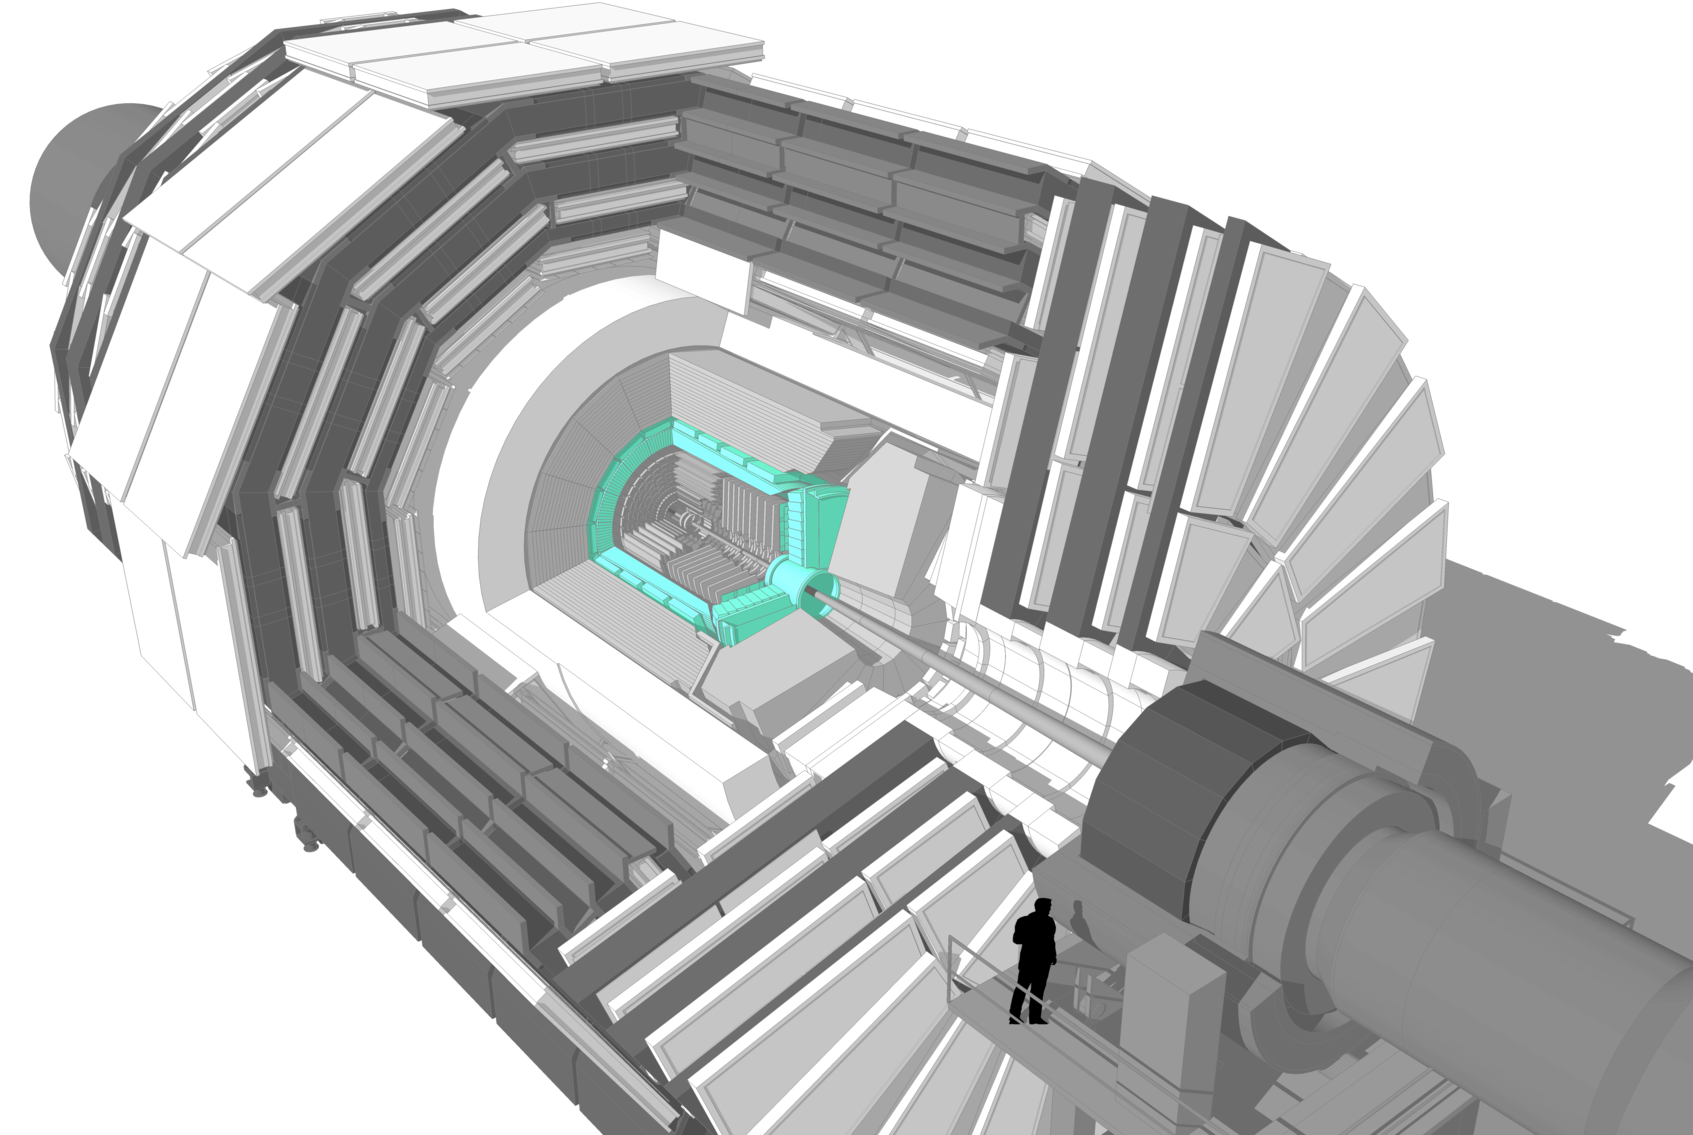
\includegraphics[width=\textwidth,height=\graphh,keepaspectratio]{\PhDthesisdir/plots_and_images/CMS_slices/from_CMS_document_11982-v2/small_cms_ecal.png}
\end{figure}
\end{minipage}
\hfill\begin{minipage}[t]{.35\textwidth}
\begin{block}{Electromagnetic CALorimeter}
\begin{itemize}
\item $\sim\num{76000}$ scintillating \ce{PbWO4} crystals
\end{itemize}
\end{block}

\begin{block}{}
$\Rightarrow$ electrons and photons are stopped, energy deposits
\end{block}
\end{minipage}
\end{frame}

\begin{frame}
\addtocounter{framenumber}{-1}
%\transdissolve
\begin{minipage}[t]{.6\textwidth}
\begin{figure}
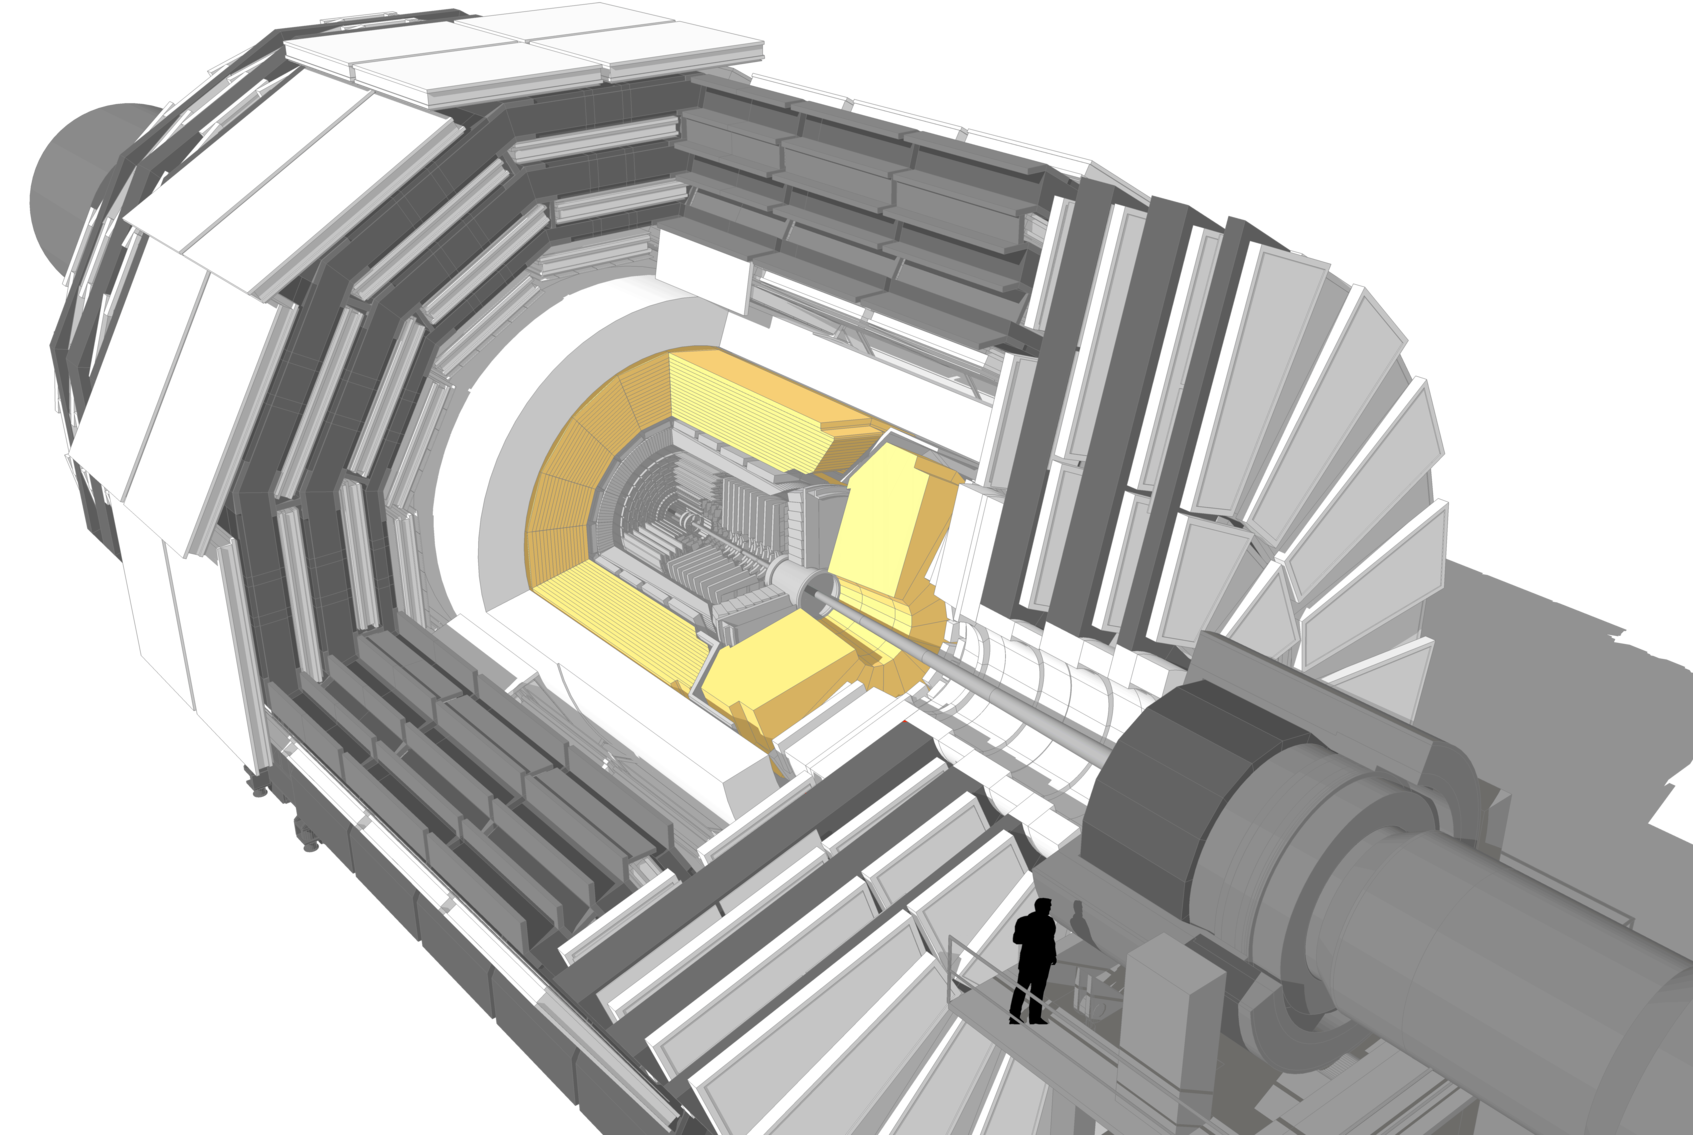
\includegraphics[width=\textwidth,height=\graphh,keepaspectratio]{\PhDthesisdir/plots_and_images/CMS_slices/from_CMS_document_11982-v2/small_cms_hcal.png}
\end{figure}
\end{minipage}
\hfill\begin{minipage}[t]{.35\textwidth}
\begin{block}{Hadronic CALorimeter (yellow)}
\begin{itemize}
\item brass + plastic scintillator, $\sim\num{7000}$ channels
\end{itemize}
\end{block}

\begin{block}{Forward CALorimeter (orange)}
\begin{itemize}
\item steel + quartz fibres, $\sim\num{2000}$ channels
\end{itemize}
\end{block}

\begin{block}{}
$\Rightarrow$ hadrons are stopped, energy deposits
\end{block}
\end{minipage}
\end{frame}

\begin{frame}
\addtocounter{framenumber}{-1}
%\transdissolve
\begin{minipage}[t]{.6\textwidth}
\begin{figure}
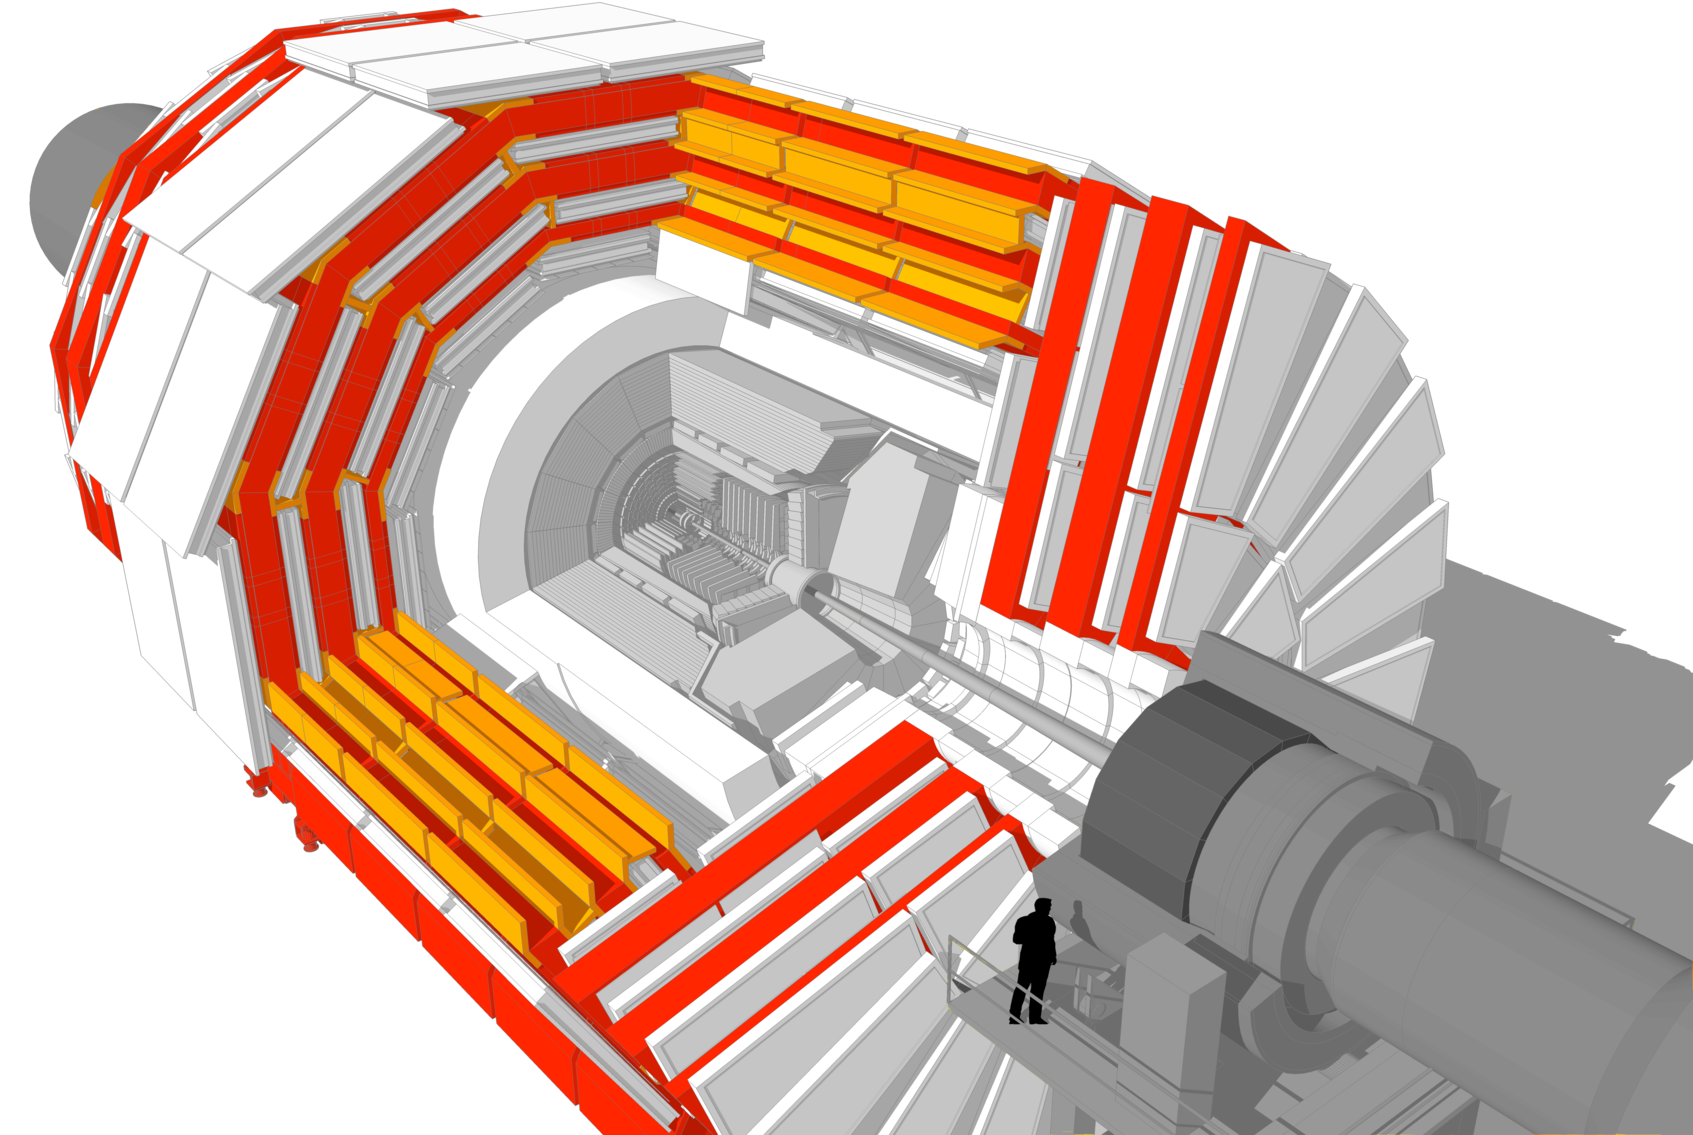
\includegraphics[width=\textwidth,height=\graphh,keepaspectratio]{\PhDthesisdir/plots_and_images/CMS_slices/from_CMS_document_11982-v2/small_cms_muons.png}
\end{figure}
\end{minipage}
\hfill\begin{minipage}[t]{.35\textwidth}
\begin{block}{Steel return yoke (red)}
\begin{itemize}
\item allows for \SI{2}{\tesla} magnetic field around the solenoid
\end{itemize}
\end{block}

\begin{block}{Muon chambers (blue-gray)}
\begin{itemize}
\item Barrel: \num{250} drift tubes, \num{480} resistive plate chambers
\item Endcaps: \num{540} cathode strip, \num{576} resistive plate chambers
\end{itemize}
\end{block}

\begin{block}{}
$\Rightarrow$ charged particles leave hits when going through (only muons do)
\end{block}
\vspace{-2\baselineskip}
\end{minipage}
\end{frame}

\begin{frame}
\addtocounter{framenumber}{-1}
%\transdissolve
\begin{minipage}[t]{.6\textwidth}
\begin{figure}
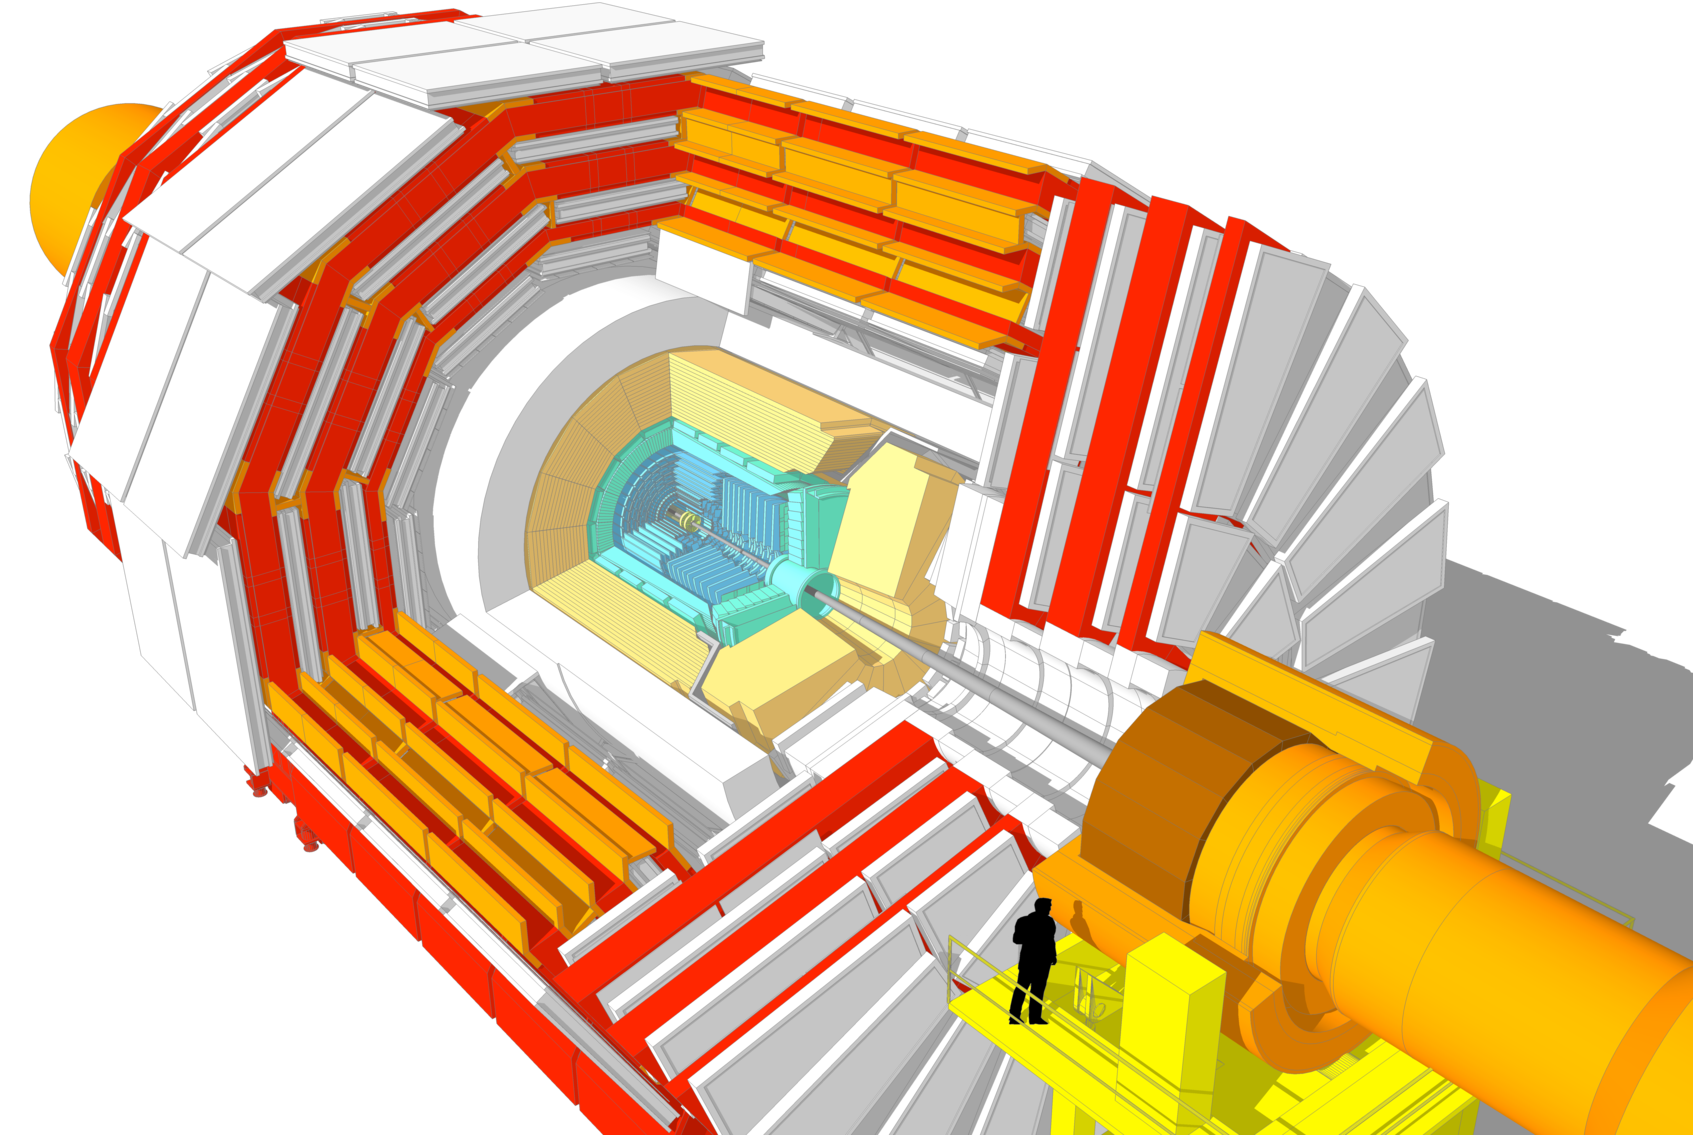
\includegraphics[width=\textwidth,height=\graphh,keepaspectratio]{\PhDthesisdir/plots_and_images/CMS_slices/from_CMS_document_11982-v2/small_cms_full_no_violet_solen.png}
\end{figure}
\end{minipage}
\hfill\begin{minipage}[t]{.35\textwidth}
\begin{block}{Sensitive parts of CMS}
Combine sub-detectors signals to determine which particles were there!
\end{block}
\end{minipage}
\end{frame}
\begin{frame}
\transdissolve
\transduration{0}
\end{frame}

\begin{frame}
\transwipe
\transduration{0}
\begin{center}
\includegraphics[width=\textwidth,height=\graphh,keepaspectratio]{\PhDthesisdir/plots_and_images/CMS_slices/own/cms_slice_CMS_parts/1-only_cms_size.tex}
\end{center}
\end{frame}

\begin{frame}
\addtocounter{framenumber}{-1}
\transdissolve[duration=2]
\transduration{0}
\begin{center}
\includegraphics[width=\textwidth,height=\graphh,keepaspectratio]{\PhDthesisdir/plots_and_images/CMS_slices/own/cms_slice_CMS_parts/2-add_trk.tex}
\end{center}
\end{frame}

\begin{frame}
\addtocounter{framenumber}{-1}
\transdissolve[duration=2]
\transduration{0}
\begin{center}
\includegraphics[width=\textwidth,height=\graphh,keepaspectratio]{\PhDthesisdir/plots_and_images/CMS_slices/own/cms_slice_CMS_parts/3-add_ECAL.tex}
\end{center}
\end{frame}

\begin{frame}
\addtocounter{framenumber}{-1}
\transdissolve[duration=2]
\transduration{0}
\begin{center}
\includegraphics[width=\textwidth,height=\graphh,keepaspectratio]{\PhDthesisdir/plots_and_images/CMS_slices/own/cms_slice_CMS_parts/4-add_HCAL.tex}
\end{center}
\end{frame}

\begin{frame}
\addtocounter{framenumber}{-1}
\transdissolve[duration=2]
\transduration{0}
\begin{center}
\includegraphics[width=\textwidth,height=\graphh,keepaspectratio]{\PhDthesisdir/plots_and_images/CMS_slices/own/cms_slice_CMS_parts/5-add_solen.tex}
\end{center}
\end{frame}

%\begin{frame}
%\addtocounter{framenumber}{-1}
%\transdissolve
%\transduration{0}
%\begin{center}
%\includegraphics[width=\textwidth,height=\graphh,keepaspectratio]{\PhDthesisdir/plots_and_images/CMS_slices/own/cms_slice_CMS_parts/6-1-add_iron_RY.tex}
%\end{center}
%\end{frame}
%
%\begin{frame}
%\addtocounter{framenumber}{-1}
%\transdissolve
%\transduration{0}
%\begin{center}
%\includegraphics[width=\textwidth,height=\graphh,keepaspectratio]{\PhDthesisdir/plots_and_images/CMS_slices/own/cms_slice_CMS_parts/6-2-add_muon1.tex}
%\end{center}
%\end{frame}
%
%\begin{frame}
%\addtocounter{framenumber}{-1}
%\transdissolve
%\transduration{0}
%\begin{center}
%\includegraphics[width=\textwidth,height=\graphh,keepaspectratio]{\PhDthesisdir/plots_and_images/CMS_slices/own/cms_slice_CMS_parts/6-3-add_muon2.tex}
%\end{center}
%\end{frame}
%
%\begin{frame}
%\addtocounter{framenumber}{-1}
%\transdissolve
%\transduration{0}
%\begin{center}
%\includegraphics[width=\textwidth,height=\graphh,keepaspectratio]{\PhDthesisdir/plots_and_images/CMS_slices/own/cms_slice_CMS_parts/6-4-add_muon3.tex}
%\end{center}
%\end{frame}

\begin{frame}
\addtocounter{framenumber}{-1}
\transdissolve[duration=2]
\transduration{0}
\begin{center}
\includegraphics[width=\textwidth,height=\graphh,keepaspectratio]{\PhDthesisdir/plots_and_images/CMS_slices/own/cms_slice_CMS_parts/6-5-add_muon4.tex}
\end{center}
\end{frame}

%\begin{frame}
%\addtocounter{framenumber}{-1}
%\transdissolve[duration=2]
%\transduration{0}
%\begin{center}
%\includegraphics[width=\textwidth,height=\graphh,keepaspectratio]{\PhDthesisdir/plots_and_images/CMS_slices/own/cms_slice_CMS_parts/7-add_B_field.tex}
%\end{center}
%\end{frame}

\begin{frame}
\addtocounter{framenumber}{-1}
\transdissolve[duration=2]
\transduration{0}
\begin{center}
\includegraphics[width=\textwidth,height=\graphh,keepaspectratio]{\PhDthesisdir/plots_and_images/CMS_slices/own/cms_slice_particles_appear/0-nothing.tex}
\end{center}
\end{frame}

%\begin{frame}
%\addtocounter{framenumber}{-1}
%\transwipe
%\transduration{0}
%\begin{center}
%\includegraphics[width=\textwidth,height=\graphh,keepaspectratio]{\PhDthesisdir/plots_and_images/CMS_slices/own/cms_slice_particles_appear/1-up_to_CH.tex}
%\end{center}
%\end{frame}
%
%\begin{frame}
%\addtocounter{framenumber}{-1}
%\transwipe
%\transduration{0}
%\begin{center}
%\includegraphics[width=\textwidth,height=\graphh,keepaspectratio]{\PhDthesisdir/plots_and_images/CMS_slices/own/cms_slice_particles_appear/2-up_to_NH.tex}
%\end{center}
%\end{frame}
%
%\begin{frame}
%\addtocounter{framenumber}{-1}
%\transwipe
%\transduration{0}
%\begin{center}
%\includegraphics[width=\textwidth,height=\graphh,keepaspectratio]{\PhDthesisdir/plots_and_images/CMS_slices/own/cms_slice_particles_appear/3-up_to_photon.tex}
%\end{center}
%\end{frame}
%
%\begin{frame}
%\addtocounter{framenumber}{-1}
%\transwipe
%\transduration{0}
%\begin{center}
%\includegraphics[width=\textwidth,height=\graphh,keepaspectratio]{\PhDthesisdir/plots_and_images/CMS_slices/own/cms_slice_particles_appear/4-up_to_ele.tex}
%\end{center}
%\end{frame}

\begin{frame}
\addtocounter{framenumber}{-1}
\transwipe
\begin{center}
\includegraphics[width=\textwidth,height=\graphh,keepaspectratio]{\PhDthesisdir/plots_and_images/CMS_slices/own/all_ptcs.tex}
\end{center}
\end{frame}
%\begin{frame}
\frametitle{Neutrinos and missing transverse energy (MET)}

\begin{center}
\begin{tikzpicture}
\def\trackerrin{.100}
\def\trackerrout{1.185}
\def\trackercolor{ltcolorgray1}

\def\ECALrin{1.290}
\def\ECALrout{1.811}
\def\ECALcolor{ltcolorgreen1}

\def\HCALrin{1.812}
\def\HCALrout{2.854}
\def\HCALcolor{ltcoloryellow3}

\def\Solenrin{2.950}
\def\Solenrout{3.800}
\def\Solencolor{ltcolorgray2}

\def\ironryrina{3.850}
\def\ironryrouta{4.000}
\def\muonrina{4.020}
\def\muonrouta{4.400}
\def\ironryrinb{4.420}
\def\ironryroutb{4.880}
\def\muonrinb{4.905}
\def\muonroutb{5.285}
\def\ironryrinc{5.300}
\def\ironryroutc{5.960}
\def\muonrinc{5.975}
\def\muonroutc{6.355}
\def\ironryrind{6.375}
\def\ironryroutd{6.980}
\def\muonrind{7.000}
\def\muonroutd{7.380}
\def\muoncolor{ltcoloryellow1}
\def\ironrycolor{ltcolorred2}

\def\printele#1{
\draw [thick, ltcolorred] (0,0) arc (#1-90:#1-90+27:3) coordinate (eledeposit);
\draw [ltcolorred] (#1-5:1.25) node {\ele};
}
\def\printmu#1{
\draw [thick, ltcolorblue] (0,0) arc (#1-90:#1-90+33:6) arc (#1-90+33:#1-90:-12) node{\mu};
\draw [ltcolorblue] (#1-7:1.5) node {\mu};
}

\def\printantiele#1{
\draw [thick, ltcolorred] (0,0) arc (#1-90:#1-90-27:-3) coordinate (eledeposit);
\draw [ltcolorred] (#1-7:1.5) node {\ele};
%\draw [ltcolorred4, ultra thick] (eledeposit)--+(#1+25:\ECALrout);
}
\def\printantimu#1{
\draw [thick, ltcolorblue] (0,0) arc (#1-90:#1-90-33:-6) arc (#1-90-33:#1-90:12);
\draw [ltcolorblue] (#1-7:1.5) node {\mu};
}

\def\printtauh#1{
\draw [thick, ltcolorgreen4] (0,0) arc (#1-90:#1-90+11:10) ;
\draw [thick, ltcolorgreen4] (0,0) arc (#1-90:#1-90+6:20) ;
\draw [thick, ltcolorgreen4] (0,0) arc (#1-90:#1-90-11:-10) ;
\draw [ltcolorgreen4] (#1-12:1.5) node {\tauh};
}
\def\printantitauh#1{
\draw [thick, ltcolorgreen4] (0,0) arc (#1-90:#1-90-11:-10) ;
\draw [thick, ltcolorgreen4] (0,0) arc (#1-90:#1-90-6:-20) ;
\draw [thick, ltcolorgreen4] (0,0) arc (#1-90:#1-90+11:10) ;
\draw [ltcolorgreen4] (#1-12:1.5) node {\tauh};
}

\def\printjetnolabel#1{
\draw [thick, ltcolororange] (0,0) arc (#1-90+10:#1-90+22+10:5) ;
\draw [thick, ltcolororange] (0,0) arc (#1-90+5:#1-90+12+5:10) ;
\draw [thick, ltcolororange] (0,0) arc (#1-90:#1-90-22:-5) ;
\draw [thick, ltcolororange] (0,0) arc (#1-90:#1-90+6:20) ;
\draw [thick, ltcolororange] (0,0) arc (#1-90+5:#1-90+8+5:10) ;
\draw [thick, ltcolororange] (0,0) arc (#1-90:#1-90-11:-10) ;
\draw [thick, ltcolororange] (0,0) arc (#1-90:#1-90+11:10) ;
}

\def\printjet#1{
\printjetnolabel{#1}
\draw [ltcolororange] (#1-25:.5) node {jet};
}

\def\printjetfake#1{
\printjet{#1}
\draw [thick, ltcolorgreen4] (0,0) arc (#1-90:#1-90+11:10) ;
\draw [thick, ltcolorgreen4] (0,0) arc (#1-90:#1-90+6:20) ;
\draw [thick, ltcolorgreen4] (0,0) arc (#1-90:#1-90-11:-10) ;
\draw [ltcolorgreen4] (#1-17:1.5) node {f.\tauh};
}

\def\printdeposit#1#2#3#4{
\fill [#1] (#2-2:#3) arc (#2-2:#2+2:#3) -- (#2+2:#4) arc (#2+2:#2-2:#4) ;
}

\def\printECALdeposit#1#2{\printdeposit{#1}{#2}{\ECALrin}{\ECALrout}}
\def\printHCALdeposit#1#2{\printdeposit{#1}{#2}{\HCALrin}{\HCALrout}}

\def\printtauhdeposit#1{
\printHCALdeposit{ltcoloryellow4}{#1+3}
\printHCALdeposit{ltcoloryellow4}{#1+5}
\printHCALdeposit{ltcoloryellow4}{#1-5}
}

\def\printjetdeposit#1{
\printHCALdeposit{ltcoloryellow4}{#1+3}
\printHCALdeposit{ltcoloryellow4}{#1+5}
\printHCALdeposit{ltcoloryellow4}{#1-5}
\printHCALdeposit{ltcoloryellow4}{#1+21}
\printHCALdeposit{ltcoloryellow4}{#1+11}
\printHCALdeposit{ltcoloryellow4}{#1-11}
}

\def\printMuChSigA#1#2{
\fill [red] (#1-7.5+20*#2:\muonrina) arc (#1-7.5+20*#2:#1+7.5+20*#2:\muonrina) -- (#1+7.5+20*#2:\muonrouta) arc (#1+7.5+20*#2:#1-7.5+20*#2:\muonrouta) ;
}
\def\printMuChSigB#1#2{
\fill [red] (#1-7.5+20*#2:\muonrinb) arc (#1-7.5+20*#2:#1+7.5+20*#2:\muonrinb) -- (#1+7.5+20*#2:\muonroutb) arc (#1+7.5+20*#2:#1-7.5+20*#2:\muonroutb) ;
}
\def\printMuChSigC#1#2{
\fill [red] (#1-7.5+20*#2:\muonrinc) arc (#1-7.5+20*#2:#1+7.5+20*#2:\muonrinc) -- (#1+7.5+20*#2:\muonroutc) arc (#1+7.5+20*#2:#1-7.5+20*#2:\muonroutc) ;
}
\def\printMuChSigD#1#2{
\fill [red] (#1-7.5+20*#2:\muonrind) arc (#1-7.5+20*#2:#1+7.5+20*#2:\muonrind) -- (#1+7.5+20*#2:\muonroutd) arc (#1+7.5+20*#2:#1-7.5+20*#2:\muonroutd) ;
}

\clip (-\graphw/2,-\graphh/2) rectangle (\graphw/2,\graphh/2);

\printjetnolabel{60}
\printjetnolabel{40}

%\draw [thick, -latex, ltcolorred] (0,0)--+(-130:\HCALrout) node [below] {\vMET};

\fill (0,0) circle (2pt);
\end{tikzpicture}
\end{center}

\end{frame}

\begin{frame}\addtocounter{framenumber}{-1}
\frametitle{Neutrinos and missing transverse energy (MET)}

\begin{center}
\begin{tikzpicture}
\def\trackerrin{.100}
\def\trackerrout{1.185}
\def\trackercolor{ltcolorgray1}

\def\ECALrin{1.290}
\def\ECALrout{1.811}
\def\ECALcolor{ltcolorgreen1}

\def\HCALrin{1.812}
\def\HCALrout{2.854}
\def\HCALcolor{ltcoloryellow3}

\def\Solenrin{2.950}
\def\Solenrout{3.800}
\def\Solencolor{ltcolorgray2}

\def\ironryrina{3.850}
\def\ironryrouta{4.000}
\def\muonrina{4.020}
\def\muonrouta{4.400}
\def\ironryrinb{4.420}
\def\ironryroutb{4.880}
\def\muonrinb{4.905}
\def\muonroutb{5.285}
\def\ironryrinc{5.300}
\def\ironryroutc{5.960}
\def\muonrinc{5.975}
\def\muonroutc{6.355}
\def\ironryrind{6.375}
\def\ironryroutd{6.980}
\def\muonrind{7.000}
\def\muonroutd{7.380}
\def\muoncolor{ltcoloryellow1}
\def\ironrycolor{ltcolorred2}

\def\printele#1{
\draw [thick, ltcolorred] (0,0) arc (#1-90:#1-90+27:3) coordinate (eledeposit);
\draw [ltcolorred] (#1-5:1.25) node {\ele};
}
\def\printmu#1{
\draw [thick, ltcolorblue] (0,0) arc (#1-90:#1-90+33:6) arc (#1-90+33:#1-90:-12) node{\mu};
\draw [ltcolorblue] (#1-7:1.5) node {\mu};
}

\def\printantiele#1{
\draw [thick, ltcolorred] (0,0) arc (#1-90:#1-90-27:-3) coordinate (eledeposit);
\draw [ltcolorred] (#1-7:1.5) node {\ele};
%\draw [ltcolorred4, ultra thick] (eledeposit)--+(#1+25:\ECALrout);
}
\def\printantimu#1{
\draw [thick, ltcolorblue] (0,0) arc (#1-90:#1-90-33:-6) arc (#1-90-33:#1-90:12);
\draw [ltcolorblue] (#1-7:1.5) node {\mu};
}

\def\printtauh#1{
\draw [thick, ltcolorgreen4] (0,0) arc (#1-90:#1-90+11:10) ;
\draw [thick, ltcolorgreen4] (0,0) arc (#1-90:#1-90+6:20) ;
\draw [thick, ltcolorgreen4] (0,0) arc (#1-90:#1-90-11:-10) ;
\draw [ltcolorgreen4] (#1-12:1.5) node {\tauh};
}
\def\printantitauh#1{
\draw [thick, ltcolorgreen4] (0,0) arc (#1-90:#1-90-11:-10) ;
\draw [thick, ltcolorgreen4] (0,0) arc (#1-90:#1-90-6:-20) ;
\draw [thick, ltcolorgreen4] (0,0) arc (#1-90:#1-90+11:10) ;
\draw [ltcolorgreen4] (#1-12:1.5) node {\tauh};
}

\def\printjetnolabel#1{
\draw [thick, ltcolororange] (0,0) arc (#1-90+10:#1-90+22+10:5) ;
\draw [thick, ltcolororange] (0,0) arc (#1-90+5:#1-90+12+5:10) ;
\draw [thick, ltcolororange] (0,0) arc (#1-90:#1-90-22:-5) ;
\draw [thick, ltcolororange] (0,0) arc (#1-90:#1-90+6:20) ;
\draw [thick, ltcolororange] (0,0) arc (#1-90+5:#1-90+8+5:10) ;
\draw [thick, ltcolororange] (0,0) arc (#1-90:#1-90-11:-10) ;
\draw [thick, ltcolororange] (0,0) arc (#1-90:#1-90+11:10) ;
}

\def\printjet#1{
\printjetnolabel{#1}
\draw [ltcolororange] (#1-25:.5) node {jet};
}

\def\printjetfake#1{
\printjet{#1}
\draw [thick, ltcolorgreen4] (0,0) arc (#1-90:#1-90+11:10) ;
\draw [thick, ltcolorgreen4] (0,0) arc (#1-90:#1-90+6:20) ;
\draw [thick, ltcolorgreen4] (0,0) arc (#1-90:#1-90-11:-10) ;
\draw [ltcolorgreen4] (#1-17:1.5) node {f.\tauh};
}

\def\printdeposit#1#2#3#4{
\fill [#1] (#2-2:#3) arc (#2-2:#2+2:#3) -- (#2+2:#4) arc (#2+2:#2-2:#4) ;
}

\def\printECALdeposit#1#2{\printdeposit{#1}{#2}{\ECALrin}{\ECALrout}}
\def\printHCALdeposit#1#2{\printdeposit{#1}{#2}{\HCALrin}{\HCALrout}}

\def\printtauhdeposit#1{
\printHCALdeposit{ltcoloryellow4}{#1+3}
\printHCALdeposit{ltcoloryellow4}{#1+5}
\printHCALdeposit{ltcoloryellow4}{#1-5}
}

\def\printjetdeposit#1{
\printHCALdeposit{ltcoloryellow4}{#1+3}
\printHCALdeposit{ltcoloryellow4}{#1+5}
\printHCALdeposit{ltcoloryellow4}{#1-5}
\printHCALdeposit{ltcoloryellow4}{#1+21}
\printHCALdeposit{ltcoloryellow4}{#1+11}
\printHCALdeposit{ltcoloryellow4}{#1-11}
}

\def\printMuChSigA#1#2{
\fill [red] (#1-7.5+20*#2:\muonrina) arc (#1-7.5+20*#2:#1+7.5+20*#2:\muonrina) -- (#1+7.5+20*#2:\muonrouta) arc (#1+7.5+20*#2:#1-7.5+20*#2:\muonrouta) ;
}
\def\printMuChSigB#1#2{
\fill [red] (#1-7.5+20*#2:\muonrinb) arc (#1-7.5+20*#2:#1+7.5+20*#2:\muonrinb) -- (#1+7.5+20*#2:\muonroutb) arc (#1+7.5+20*#2:#1-7.5+20*#2:\muonroutb) ;
}
\def\printMuChSigC#1#2{
\fill [red] (#1-7.5+20*#2:\muonrinc) arc (#1-7.5+20*#2:#1+7.5+20*#2:\muonrinc) -- (#1+7.5+20*#2:\muonroutc) arc (#1+7.5+20*#2:#1-7.5+20*#2:\muonroutc) ;
}
\def\printMuChSigD#1#2{
\fill [red] (#1-7.5+20*#2:\muonrind) arc (#1-7.5+20*#2:#1+7.5+20*#2:\muonrind) -- (#1+7.5+20*#2:\muonroutd) arc (#1+7.5+20*#2:#1-7.5+20*#2:\muonroutd) ;
}

\clip (-\graphw/2,-\graphh/2) rectangle (\graphw/2,\graphh/2);

\printjetnolabel{60}
\printjetnolabel{40}

\draw [thick, -latex, ltcolorred] (0,0)--+(-130:\HCALrout) node [below] {\vMET};

\fill (0,0) circle (2pt);
\end{tikzpicture}
\end{center}

\end{frame}

\begin{frame}
\frametitle{Event display: $\higgs\to\tau\tau\to\mu\tauh$ candidate}
\vfill
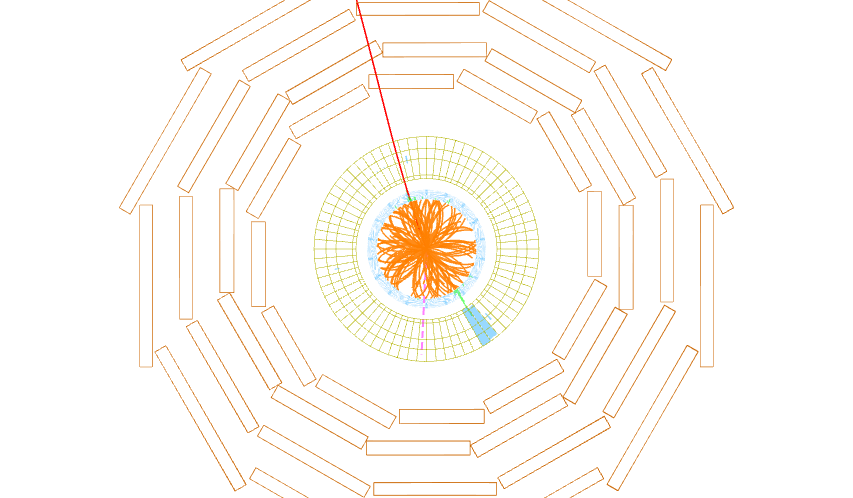
\includegraphics[width=\graphw,height=\graphh,keepaspectratio]{\PhDthesisdir/tex/slides/SM_MSSM_HTT_pheno/event_display/Event_1429090375_xy_white_struct_tracks.png}

\vfill

{\tiny
CMS record, Aug. 18, 2012, 14:37:39.352716 GMT
\qquad
Run 201191, Event 1429090375, LS 1071, xy plane.
}
\end{frame}
